\documentclass[11pt]{amsart}

\usepackage[T1]{fontenc}
\usepackage{lmodern}
\usepackage{amssymb,amsmath}
\usepackage{graphicx}
\usepackage{enumitem}
\usepackage{booktabs}
\usepackage[dvipsnames]{xcolor}
\usepackage[margin=1.15in]{geometry}
\usepackage{xurl}
\usepackage[colorlinks=true,linkcolor=blue!50!black,citecolor=blue!50!black,urlcolor=blue!50!black]{hyperref}

\newtheorem{theorem}{Theorem}[section]
\newtheorem{proposition}[theorem]{Proposition}
\newtheorem{lemma}[theorem]{Lemma}
\newtheorem{corollary}[theorem]{Corollary}
\newtheorem{conjecture}[theorem]{Conjecture}
\newtheorem{problem}[theorem]{Problem}
\newtheorem{introthm}{Theorem}
\renewcommand{\theintrothm}{\Alph{introthm}}
\newtheorem*{shankarthm}{Theorem}
\newtheorem*{shankarconj}{Conjecture}
\theoremstyle{definition}
\newtheorem{definition}[theorem]{Definition}
\newtheorem{example}[theorem]{Example}
\theoremstyle{remark}
\newtheorem{remark}[theorem]{Remark}

\numberwithin{equation}{section}

\newcommand{\F}{\mathbb{F}}
\newcommand{\cA}{\mathcal{A}}
\newcommand{\cF}{\mathcal{F}}
\newcommand{\cG}{\mathcal{G}}
\newcommand{\cK}{\mathcal{K}}
\newcommand{\cP}{\mathcal{P}}
\newcommand{\cQ}{\mathcal{Q}}
\newcommand{\Iv}[1]{[\,#1\,]}
\DeclareMathOperator{\wt}{w}
\DeclareMathOperator{\rank}{rank}
\DeclareMathOperator{\Meven}{M_{ev}}
\DeclareMathOperator{\Modd}{M_{od}}
\hypersetup{pdftitle={Catalan Rigidity of Even Lattice Paths},pdfauthor={Deep Bhattacharjee}}
\providecommand{\doi}[1]{\href{https://doi.org/#1}{doi:\nolinkurl{#1}}}

\begin{document}

\title{Catalan Rigidity of Even Lattice Paths}

\author{Deep Bhattacharjee}
\address{Formerly, Electro-Gravitational Space Propulsion Laboratory (EGSPL),\newline Bhubaneswar, Odisha 751030, India\newline
Formerly, University of Calcutta (Heramba Chandra College),\newline 23/49 Gariahat Road, Golpark, Kolkata 700029, West Bengal, India}
\email{d.bhattacharjee@erl-forschung.de}
\email{itsdeep@live.com}
\email{egspl@proton.me}
\urladdr{https://orcid.org/0000-0003-0466-750X}
\thanks{Corresponding author: Deep Bhattacharjee,\\ \href{mailto:d.bhattacharjee@erl-forschung.de}{d.bhattacharjee@erl-forschung.de}; ORCID \href{https://orcid.org/0000-0003-0466-750X}{\mbox{0000-0003-0466-750X}}}

\subjclass[2020]{Primary 05A15, 05D05; Secondary 05C50, 15B33}
\keywords{lattice paths, Catalan numbers, parity intersection theorems}

\begin{abstract}
A family of North--East lattice paths from $(0,0)$ to $(n,n)$ in which any two paths share an even number of edges has at most $2^n$ members. We prove Shankar's conjecture that exactly $C_n$ families attain this bound, one for each noncrossing perfect matching, by classifying all equality cases of the underlying inequality. We also compute the binary rank of every grid graph and bound parity families of paths in every rectangle.
\end{abstract}

\maketitle

\section{Introduction}\label{sec:intro}

\subsection{Intersection theorems for sets and for paths}

Two classical theorems describe families of subsets of an $n$-element set under parity conditions on intersections. If every member has odd size and any two members meet in an even number of points, the family has at most $n$ members (Oddtown).\footnote{The whole argument is short. Let $v_1,\dots,v_N\in\F_2^n$ be the indicator vectors of the members. The product $v_s\cdot v_s$ is the size of the $s$th member modulo $2$, which is $1$, and for $s\ne t$ the product $v_s\cdot v_t$ is the size of an intersection modulo $2$, which is $0$; so the Gram matrix of $v_1,\dots,v_N$ over $\F_2$ is the identity. If $\sum_s\lambda_sv_s=0$, taking the product with $v_t$ gives $\lambda_t=0$. The vectors are therefore linearly independent and $N\le n$, with equality for the $n$ singletons. The polynomial bounds of Theorem~\ref{thm:D} come from the same comparison of a Gram matrix with the rank of the ambient form.} If all sizes and all pairwise intersections are even, the family has at most $2^{\lfloor n/2\rfloor}$ members (Eventown); this is due to Berlekamp~\cite{Be} and Graver~\cite{Gr}, and both theorems are now standard examples of the linear algebra method in extremal combinatorics~\cite{FW,FO}. A maximal Eventown family is closed under symmetric difference, since the symmetric difference of two members again has even size and even intersection with every member; so it is a self-orthogonal subspace of $\F_2^n$, and the bound is the dimension count for such subspaces.\footnote{The standard form on $\F_2^n$ is nondegenerate, so $\dim U+\dim U^\perp=n$ for every subspace $U$. If $U\subseteq U^\perp$, then $2\dim U\le n$ and $|U|\le2^{\lfloor n/2\rfloor}$. The bound is attained by splitting $[n]$ into $\lfloor n/2\rfloor$ disjoint pairs, with one point left over when $n$ is odd, and taking all unions of pairs.}

Shankar~\cite{Sh} asked for analogues in which the ground set is replaced by the edges of a grid and the sets by lattice paths. A \emph{lattice path} from $(0,0)$ to $(a,b)$ is a sequence of $a+b$ unit steps, each either north ($N$) or east ($E$); two paths \emph{intersect} in their common edges. The idea of measuring the intersection of two paths by their common edges is due to Hiranya Dey, as Shankar records~\cite{Sh}. For square grids, Shankar proved the following two theorems.

\begin{shankarthm}[Shankar {\cite{Sh}}]
Let $\cF$ be a family of lattice paths from $(0,0)$ to $(n,n)$.
\begin{enumerate}[label=\textup{(\roman*)}]
\item If any two distinct paths of $\cF$ have an even number of common edges, then $|\cF|\le 2^n$, and the bound is attained.
\item If any two distinct paths of $\cF$ have an odd number of common edges, then $|\cF|\le n(n-1)+1$, and $|\cF|$ can be of order $n^2$.
\end{enumerate}
\end{shankarthm}

The bound in (i) is attained by many families. A perfect matching $M$ of $[2n]=\{1,\dots,2n\}$ is \emph{noncrossing} if it contains no two pairs $\{p,q\}$, $\{p',q'\}$ with $p<p'<q<q'$; there are $C_n=\frac1{n+1}\binom{2n}{n}$ of them~\cite{St,StEC2}.\footnote{The first values are $C_1,\dots,C_6=1,2,5,14,42,132$. A noncrossing perfect matching of $[2n]$ is the same object as a Dyck path with $2n$ steps: reading $1,\dots,2n$ from left to right, write an up step at the smaller point of each pair and a down step at the larger one. Because no two pairs cross, the pairs nest like brackets, and the matching is recovered from the path by pairing each down step with the nearest unmatched up step before it. Stanley's monograph~\cite{St} collects more than two hundred further objects counted by $C_n$.} For such $M$ let $\cF_M$ be the set of words $w\in\{E,N\}^{2n}$ with $w_p\ne w_q$ for every pair $\{p,q\}\in M$. Each pair can be filled with $EN$ or with $NE$ independently, so $|\cF_M|=2^n$, and every word of $\cF_M$ has $n$ letters of each kind, so it describes a path from $(0,0)$ to $(n,n)$. Shankar showed that any two paths of $\cF_M$ share an even number of edges, that different matchings give different families, and conjectured that there are no other extremal families~\cite[Conjecture~4.1]{Sh}; he checked this for $n\le5$. Figure~\ref{fig:families} shows the two families for $n=2$.

\begin{shankarconj}[Shankar]
There are exactly $C_n$ families of $2^n$ lattice paths from $(0,0)$ to $(n,n)$ in which every two distinct paths have an even number of common edges.
\end{shankarconj}

\begin{figure}[ht]
\centering
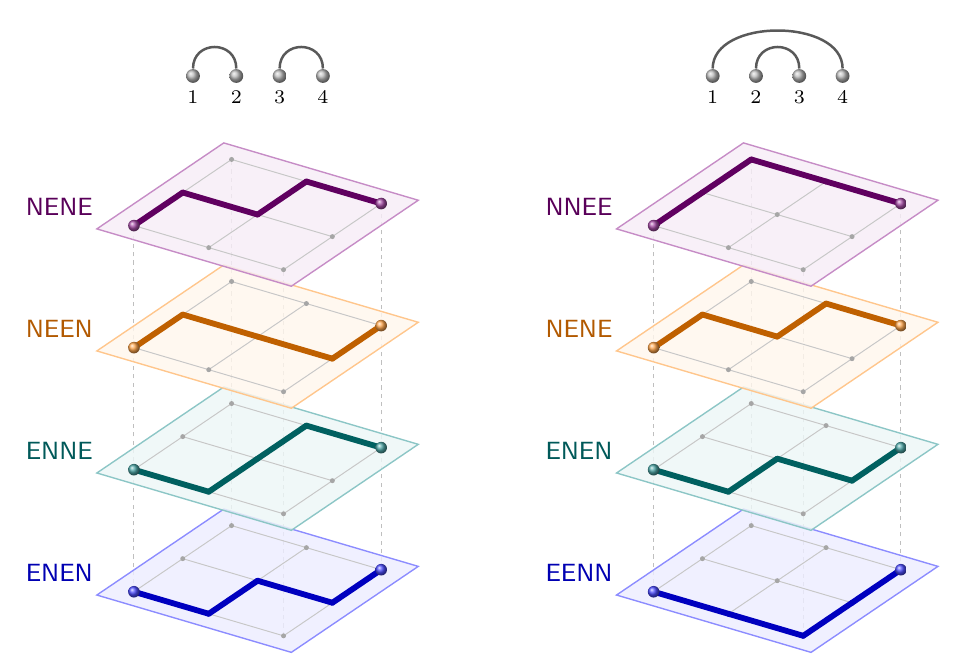
\includegraphics[width=0.86\textwidth]{families.png}
\caption{The two extremal families for $n=2$. On the left $M=\{\{1,2\},\{3,4\}\}$, on the right $M=\{\{1,4\},\{2,3\}\}$; each family has four paths, drawn on four parallel copies of the grid $\{0,1,2\}^2$. Any two paths of one family share $0$ or $2$ edges.}
\label{fig:families}
\end{figure}

\subsection{The main theorem}

We prove the conjecture.

\begin{introthm}\label{thm:A}
Let $\cF$ be a family of $2^n$ lattice paths from $(0,0)$ to $(n,n)$ in which every two distinct paths have an even number of common edges. Then $\cF=\cF_M$ for a unique noncrossing perfect matching $M$ of $[2n]$. In particular, there are exactly $C_n$ such families.
\end{introthm}

Shankar's proof of the bound $2^n$ passes through an inequality for collections of sets of binary words~\cite[Lemma~2.3]{Sh}, proved by deleting the last letter of every word. Theorem~\ref{thm:A} is a consequence of a complete description of the collections for which this inequality is an equality. To state it, identify $N$ with $1$ and $E$ with $0$, so that a path with $m$ steps is a word in $L(m)=\{0,1\}^m$. The \emph{weight} $\wt(x)$ of $x\in L(m)$ is its number of letters $1$, and $x_{<i}=x_1\cdots x_{i-1}$. For $x,y\in L(m)$ put
\[
B_m(x,y)=\#\{i\in[m]:\ x_i=y_i\ \text{and}\ \wt(x_{<i})=\wt(y_{<i})\}\bmod 2\ \in\F_2 .
\]
By~\eqref{eq:common} below, $B_m(x,y)$ is the parity of the number of common edges of the two paths.\footnote{The two conditions say that the $i$th steps of the two paths start at the same lattice point and go in the same direction, which is exactly when they are the same edge.}

\begin{definition}\label{def:admissible}
An \emph{admissible system of length $m$} is a finite collection $\cA$ of pairwise disjoint nonempty subsets of $L(m)$, its \emph{classes}, such that
\begin{enumerate}[label=\textup{(A\arabic*)}]
\item all words in a class have the same weight;
\item $B_m(x,y)=m$ in $\F_2$ whenever $x$ and $y$ lie in the same class;
\item for distinct classes $A$ and $A'$, the function $B_m$ is constant on $A\times A'$.
\end{enumerate}
We write $\|\cA\|=\sum_{A\in\cA}|A|^2$ and call $\cA$ \emph{extremal} if $\|\cA\|=2^m$.
\end{definition}

Shankar's inequality states that $\|\cA\|\le 2^m$ for every admissible system of length $m$; we prove it again as Proposition~\ref{prop:inequality}, since its equality case is our starting point.\footnote{Condition (A2) includes the case $x=y$. Since $B_m(x,x)=m$ for every word, (A2) is automatic for $x=y$, and for $x\ne y$ it says that the two paths share a number of edges congruent to $m$ modulo $2$.} The extremal systems are described by noncrossing partial matchings in which no unmatched point lies under an arc.

\begin{definition}\label{def:skeleton}
A \emph{skeleton} of $[m]$ is a pair $(M,S)$, where $M$ is a set of pairwise disjoint two-element subsets of $[m]$, the \emph{arcs}, and $S=[m]\setminus\bigcup M$ is the set of \emph{free points}, such that
\begin{enumerate}[label=(\alph*)]
\item no two arcs cross: there are no arcs $\{p,q\}$, $\{p',q'\}$ with $p<p'<q<q'$;
\item no free point lies under an arc: there are no $s\in S$ and $\{p,q\}\in M$ with $p<s<q$.
\end{enumerate}
Let $s_1<\dots<s_k$ be the free points. For $a\in L(k)$ the class $C_a=C_a(M,S)$ consists of the words $x\in L(m)$ with $x_p\ne x_q$ for every arc $\{p,q\}$ and $x_{s_j}=a_j$ for $1\le j\le k$. The \emph{skeleton system} of $(M,S)$ is $\Sigma(M,S)=\{C_a(M,S):\ a\in L(k)\}$.
\end{definition}

\begin{introthm}\label{thm:B}
An admissible system of length $m$ is extremal if and only if it is the skeleton system $\Sigma(M,S)$ of a skeleton $(M,S)$ of $[m]$. Different skeletons give different systems, and the number of extremal admissible systems of length $m$ is $\binom{m}{\lfloor m/2\rfloor}$.
\end{introthm}

A family as in Theorem~\ref{thm:A} is an extremal system of length $2n$ with a single class, and Theorem~\ref{thm:B} forces it to be $\Sigma(M,\varnothing)=\{\cF_M\}$. Figure~\ref{fig:skeleton} shows a skeleton of $[11]$ and the lattice path that encodes it in the count of Theorem~\ref{thm:B}.

\begin{figure}[ht]
\centering
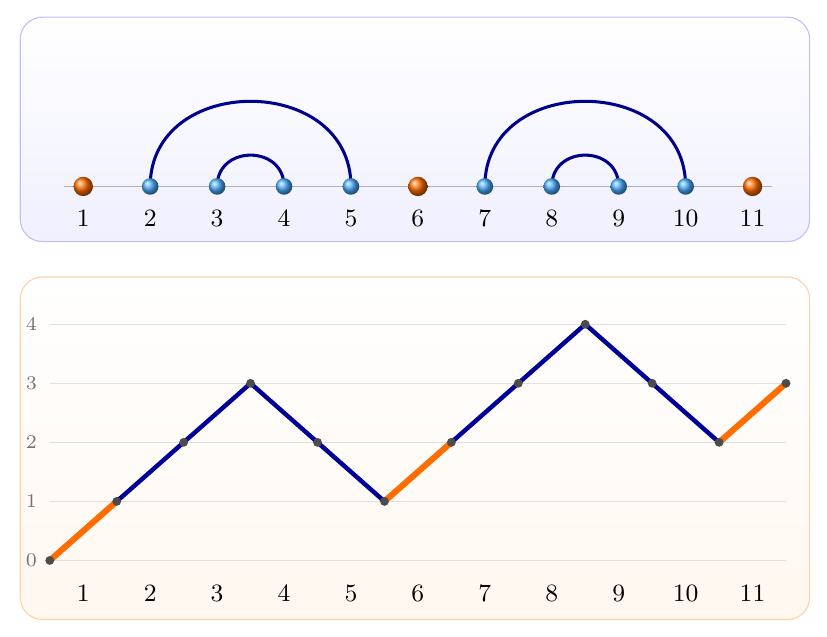
\includegraphics[width=0.8\textwidth]{skeleton.png}
\caption{Top: the skeleton of $[11]$ with arcs $\{2,5\},\{3,4\},\{7,10\},\{8,9\}$ and free points $1,6,11$. Its system has $2^3$ classes of $2^4$ words; for example $C_{101}$ consists of the words $1\,x_2x_3\bar x_3\bar x_2\,0\,x_7x_8\bar x_8\bar x_7\,1$, where $\bar x=1-x$. Bottom: the nonnegative $\pm1$ sequence attached to it in Section~\ref{sec:count}; free points and left ends of arcs are up steps.}
\label{fig:skeleton}
\end{figure}

\subsection{Rectangles, odd lengths and odd intersections}

The second half of the paper treats paths from $(0,0)$ to $(a,b)$ and both parities. For $a,b\ge0$ let $\Meven(a,b)$ and $\Modd(a,b)$ be the largest sizes of families of paths from $(0,0)$ to $(a,b)$ in which every two distinct paths share an even, respectively odd, number of edges. Shankar's theorems give $\Meven(n,n)=2^n$ and $\Modd(n,n)\le n(n-1)+1$.

The behaviour depends on the length $m=a+b$. When the parity required of pairwise intersections agrees with the parity of $m$, the family is a one-class admissible system, and the bound is exponential. When it disagrees, the Gram matrix of the family over $\F_2$ has full or nearly full rank, and the bound is polynomial; it is governed by the rank of the adjacency matrix of a grid graph, which we compute exactly.

\begin{introthm}\label{thm:C}
Let $A_{a,b}$ be the adjacency matrix of the $a\times b$ grid graph $P_a\,\square\,P_b$.\footnote{The vertices of $P_a\,\square\,P_b$ are the pairs $(i,j)$ with $1\le i\le a$ and $1\le j\le b$, and two vertices are adjacent when they agree in one coordinate and differ by $1$ in the other. It is convenient to see the vertices as the $ab$ unit cells of an $a\times b$ rectangle, two cells being adjacent when they share a side. This is why the matrix governs lattice paths: two distinct cell boundaries share exactly one edge when the cells are adjacent and none otherwise, so $A_{a,b}$ is the matrix of common-edge parities of the cell boundaries (Lemma~\ref{lem:basis}).} Then
\[
\rank_{\F_2}A_{a,b}=ab-\gcd(a+1,b+1)+1 .
\]
\end{introthm}

For $a=b$ this is the value $n(n-1)$ found by Shankar~\cite{Sh}. Kernels of such matrices over $\F_2$ are the subject of the ``$\sigma$-game'' and ``lights out'' literature, where they are studied through Chebyshev-type polynomials~\cite{Sutner89,Sutner00,GKT};\footnote{In the $\sigma$-game on a graph each vertex carries a lamp, and pressing a vertex switches the lamps of all its neighbours; in the $\sigma^+$-game, also called lights out, it also switches its own lamp. A pattern of lamps can be produced from the dark state exactly when its indicator vector lies in the column space of the adjacency matrix $A$, respectively of $A+I$, over $\F_2$. So $2^{\rank A}$ patterns are reachable in the $\sigma$-game, and by Theorem~\ref{thm:C} the $a\times b$ grid has $2^{ab-\gcd(a+1,b+1)+1}$ of them.} we give a short self-contained proof.

\begin{introthm}\label{thm:D}
Let $a,b\ge1$, $m=a+b$, and $r=ab-\gcd(a+1,b+1)+1$.
\begin{enumerate}[label=\textup{(\roman*)}]
\item If $m$ is even, then $2^{\min(a,b)}\le\Meven(a,b)\le 2^{m/2}$, with equality on the right if and only if $a=b$; and $\Modd(a,b)\le r+3$.
\item If $m$ is odd, then $2^{\min(a,b)}\le\Modd(a,b)<2^{m/2}$; and $\Meven(a,b)\le r+2$.
\item Appending a step to every path of a family reverses the parity of all pairwise intersections.\footnote{If every path receives a final step $E$, all the new paths pass through the same last edge, from $(a,b)$ to $(a+1,b)$, and no other edge is added. Each pairwise number of common edges therefore grows by exactly one, which reverses its parity. A final step $N$ acts in the same way through the edge from $(a,b)$ to $(a,b+1)$.} Hence $\Modd(a+1,b),\Modd(a,b+1)\ge\Meven(a,b)$ and $\Meven(a+1,b),\Meven(a,b+1)\ge\Modd(a,b)$.
\end{enumerate}
\end{introthm}

For paths from $(0,0)$ to $(n+1,n)$, pairwise odd families behave like the even families of the square, and the Catalan numbers appear again.

\begin{introthm}\label{thm:E}
For every $n\ge1$ there are at least $C_{n+1}$ distinct families of $2^n$ lattice paths from $(0,0)$ to $(n+1,n)$ in which every two distinct paths share an odd number of edges, and $2^n\le\Modd(n+1,n)<2^{n+1/2}$.\footnote{Since $2^{n+1/2}=\sqrt2\cdot2^n$, the theorem determines $\Modd(n+1,n)$ up to a factor smaller than $\sqrt2\approx1.414$. Conjecture~\ref{conj:oddcatalan} asserts that the lower bound is the exact value.}
\end{introthm}

We conjecture that $\Modd(n+1,n)=2^n$ and that the $C_{n+1}$ families of Theorem~\ref{thm:E} are the only extremal ones (Conjecture~\ref{conj:oddcatalan}); an exhaustive search confirms the value for $n\le5$ and the count for $n\le4$. The value $2^n$ would follow from a statement in which the endpoints are free: a set of paths of odd length $m$ from $(0,0)$ in which every two share an odd number of edges has at most $2^{(m-1)/2}$ elements (Conjecture~\ref{conj:freeend}, Proposition~\ref{prop:freeend}, Figure~\ref{fig:freeend}); we verify this statement for $m\le9$.

Finally we return to Shankar's odd problem for the square. An exhaustive search gives $\Modd(n,n)=1,2,3,6,10,16$ for $n=1,\dots,6$, and explicit families give $\Modd(7,7)\ge20$ and $\Modd(8,8)\ge28$. The constructions of~\cite{Sh} give $k^2$ for $n=2k$ and $k(k+2)$ for $n=2k+1$, that is $9$, $15$ and $16$ for $n=6,7,8$; so the leading constant $\tfrac14$ of those constructions is not the truth.\footnote{For $n=2k$ the construction has $k^2=n^2/4$ paths, and for $n=2k+1$ it has $k(k+2)=(n^2+2n-3)/4$; in both cases the size is $n^2/4+O(n)$. The values $16$, $20$ and $28$ found for $n=6,7,8$ are close to $\binom n2=15,21,28$, which is $n^2/2+O(n)$, while the upper bound $n(n-1)+1$ is $n^2+O(n)$. Figure~\ref{fig:oddvalues} compares the three curves.} The families are listed in Appendix~\ref{app:families}.

For two rows of cells, where Theorem~\ref{thm:D} leaves a gap between $4$ and $2^{(a+2)/2}$ for one parity and gives only an upper bound close to $2a$ for the other, we give explicit families: of size $\lfloor a/2\rfloor+3$ when $a+2$ has the parity of the intersections, and of size about $5a/4$ otherwise (Theorem~\ref{thm:tworows}, Figure~\ref{fig:tworows}). An exhaustive search shows that they are optimal for $a\le22$.

\subsection{Method and organisation}

The proof of Theorem~\ref{thm:B} follows Shankar's induction, which deletes the last letter of every word. In Section~\ref{sec:induction} we show that for an extremal system the two systems of length $m-1$ produced by the induction coincide, so that by induction they form one skeleton system, and the system of length $m$ is obtained from it by grouping some of its classes in pairs. Section~\ref{sec:star} proves a rigidity statement, Lemma~\ref{lem:star}, for two words of adjacent weights that no word of a third weight can tell apart; it rests on the effect of moving a path across one unit square. In Section~\ref{sec:groupings} we show that only two groupings are possible, and each gives a skeleton system of length $m$. Section~\ref{sec:count} proves Theorem~\ref{thm:A} and counts skeletons by a reflection argument. Section~\ref{sec:rank} proves Theorem~\ref{thm:C}, Section~\ref{sec:rect} proves Theorems~\ref{thm:D} and~\ref{thm:E}, and Section~\ref{sec:open} collects the problems that remain and reduces the odd Catalan problem to paths with free endpoints. Appendix~\ref{app:comp} describes the computations and Appendix~\ref{app:families} lists the families.

The paper is self-contained: every result is proved here, and the computations of Appendix~\ref{app:comp} are described in enough detail to be repeated. Standard references for lattice path enumeration and noncrossing structures are~\cite{Kr,De,Si,Kre}.

\section{Words, paths and skeletons}\label{sec:skeletons}

\subsection{Common edges}

For a word $x\in L(m)$ the $i$th step of its path starts at the point $(i-1-\wt(x_{<i}),\wt(x_{<i}))$ and goes north if $x_i=1$ and east if $x_i=0$. A point $(u,v)$ has \emph{level} $u+v$, so the $i$th step of every path starts at level $i-1$ and ends at level $i$. Two steps can therefore be the same edge only if they have the same index $i$, and then they are the same edge exactly when they start at the same point and go in the same direction. Writing $E(x)$ for the set of edges of the path of $x$, we obtain
\begin{equation}\label{eq:common}
|E(x)\cap E(y)|=\#\{i\in[m]:\ x_i=y_i\ \text{and}\ \wt(x_{<i})=\wt(y_{<i})\},
\end{equation}
so that $B_m(x,y)\equiv|E(x)\cap E(y)|\pmod 2$. Throughout, $\Iv{P}\in\F_2$ is $1$ if the statement $P$ holds and $0$ otherwise, and for a set $X\subseteq L(m-1)$ and $e\in\{0,1\}$ we write $Xe=\{xe:\ x\in X\}\subseteq L(m)$. A path from $(0,0)$ to $(a,b)$ is a word of length $a+b$ and weight $b$.

\begin{lemma}\label{lem:basic}
\textup{(a)} $B_m(x,x)=m$ for every $x\in L(m)$, and $B_m(x,y)=B_m(y,x)$.

\textup{(b)} For $x,y\in L(m-1)$ and $e,e'\in\{0,1\}$,
\[
B_m(xe,ye')=B_{m-1}(x,y)+\Iv{e=e'}\,\Iv{\wt(x)=\wt(y)} .
\]
\end{lemma}

\begin{proof}
In (a) every position counts, and the definition is symmetric. In (b) the first $m-1$ positions contribute $B_{m-1}(x,y)$, and position $m$ counts exactly when $e=e'$ and $\wt(x)=\wt(y)$, since $\wt(x)$ and $\wt(y)$ are the weights of the prefixes $(xe)_{<m}$ and $(ye')_{<m}$.
\end{proof}

A subcollection of an admissible system is again admissible, and the empty collection is admissible. If $x$ and $y$ have equal length and equal weight, Lemma~\ref{lem:basic}(b) shows that appending the same letter to both changes $B$ by $1$; this simple remark will be used in Section~\ref{sec:rect} to pass between the two parities.

\subsection{Skeleton systems are extremal}

\begin{proposition}\label{prop:skeleton}
Let $(M,S)$ be a skeleton of $[m]$ with $k$ free points, and let $a,a'\in L(k)$, $x\in C_a$ and $y\in C_{a'}$. Then
\[
\wt(x)=|M|+\wt(a)\qquad\text{and}\qquad B_m(x,y)=B_k(a,a').
\]
Consequently $\Sigma(M,S)$ is an extremal admissible system of length $m$, and the skeleton $(M,S)$ can be recovered from the union of the classes of $\Sigma(M,S)$.
\end{proposition}

\begin{proof}
Each arc carries exactly one letter $1$, so $\wt(x)=|M|+\wt(a)$. Put $\Delta_i=\wt(x_{<i})-\wt(y_{<i})$, so that position $i$ counts in $B_m(x,y)$ when $x_i=y_i$ and $\Delta_i=0$.

Let $s=s_j$ be a free point. By condition (b) of Definition~\ref{def:skeleton}, every arc lies entirely before $s$ or entirely after it, and each arc before $s$ contributes one letter $1$ to $x_{<s}$ and one to $y_{<s}$. The free points before $s$ are $s_1,\dots,s_{j-1}$, where $x$ reads $a_1,\dots,a_{j-1}$ and $y$ reads $a'_1,\dots,a'_{j-1}$. Hence $\Delta_s=\wt(a_{<j})-\wt(a'_{<j})$, and since $x_s=a_j$ and $y_s=a'_j$, position $s$ counts in $B_m(x,y)$ exactly when position $j$ counts in $B_k(a,a')$.

Let $\{p,q\}$ be an arc with $p<q$. By conditions (a) and (b), each position strictly between $p$ and $q$ lies on an arc, and that arc lies strictly between $p$ and $q$: it cannot cross $\{p,q\}$, and it cannot contain $p$ or $q$. Each such arc adds one letter $1$ to $x$ and one to $y$, so $\Delta_q=\Delta_p+x_p-y_p$. If $x_p=y_p$, then $x_q=y_q$ and $\Delta_q=\Delta_p$, so positions $p$ and $q$ both count or both do not. If $x_p\ne y_p$, then $x_q\ne y_q$ and neither counts. In either case the arc contributes an even number. Adding the contributions of the free points and the arcs gives $B_m(x,y)=B_k(a,a')$.

The classes $C_a$ are nonempty, pairwise disjoint and of size $2^{|M|}$. By the two identities, the words of $C_a$ have weight $|M|+\wt(a)$, $B_m$ is constant on $C_a\times C_{a'}$, and on $C_a\times C_a$ it equals $B_k(a,a)=k=m-2|M|$ by Lemma~\ref{lem:basic}(a), which is $m$ in $\F_2$. So $\Sigma(M,S)$ is admissible, and $\|\Sigma(M,S)\|=2^k\cdot 4^{|M|}=2^m$.

Finally, let $U$ be the union of the classes. Two positions $p\ne q$ satisfy $x_p\ne x_q$ for all $x\in U$ exactly when $\{p,q\}\in M$: if $p$ and $q$ lie on different arcs, or one of them is free, the letters at $p$ and $q$ can be chosen independently, and in particular equal. So $U$ determines $M$, and $S$ is the complement of $\bigcup M$.
\end{proof}

\begin{example}\label{ex:smallm}
For $m=2$ there are two skeletons: one arc $\{1,2\}$, whose system is $\{\{01,10\}\}$, and two free points, whose system consists of the four singletons $\{00\},\{01\},\{10\},\{11\}$. Indeed $B_2(01,10)=0$, and on singletons (A2) and (A3) hold trivially. For $m=3$ there are three skeletons: the arc $\{1,2\}$ with the free point $3$, the arc $\{2,3\}$ with the free point $1$, and three free points; the pair $\{1,3\}$ with the free point $2$ is not a skeleton, because $2$ lies under the arc. This agrees with $\binom{2}{1}=2$ and $\binom{3}{1}=3$.
\end{example}

\section{The induction step}\label{sec:induction}

In this section $\cA=\{A_1,\dots,A_r\}$ is an admissible system of length $m\ge1$. For $1\le i\le r$ and $e\in\{0,1\}$ let
\[
B_i^e=\{x\in L(m-1):\ xe\in A_i\},
\]
so that $A_i=B_i^0 0\cup B_i^1 1$. Let $I$ be the set of indices $i$ with $B_i^0\ne\varnothing$ and $B_i^1\ne\varnothing$, and, following Shankar, put
\[
\cG_0=\{B_i^0:\ B_i^0\ne\varnothing\}\cup\{B_i^1:\ i\in I\},\qquad
\cG_1=\{B_i^1:\ B_i^1\ne\varnothing\}\cup\{B_i^0:\ i\in I\}.
\]
So $\cG_0$ keeps the prefixes of the words ending in $0$, and adds the prefixes of the words ending in $1$ only from those classes that contain words of both kinds; $\cG_1$ is defined symmetrically. For a collection $\mathcal X$ of finite sets write $\|\mathcal X\|=\sum_{X\in\mathcal X}|X|^2$. Figure~\ref{fig:induction} illustrates the construction.

\begin{figure}[ht]
\centering
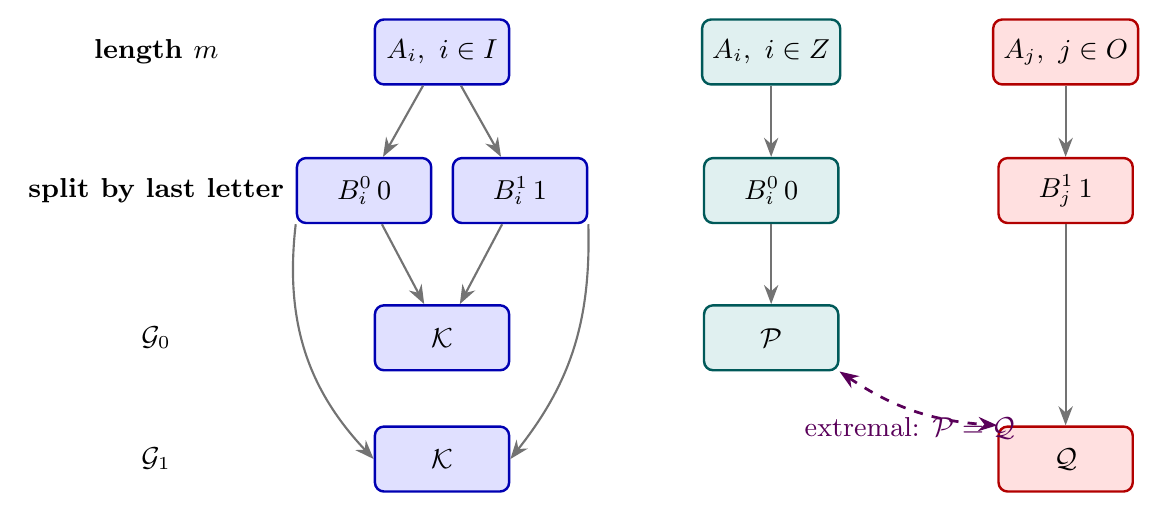
\includegraphics[width=0.92\textwidth]{fig_induction.png}
\caption{The induction step. Each class $A_i$ of length $m$ splits by its last letter into $B_i^0 0$ and $B_i^1 1$. Classes with both parts nonempty (indices in $I$) send both parts to $\cG_0$ and to $\cG_1$; classes ending only in $0$ (indices in $Z$) feed $\cG_0$, classes ending only in $1$ (indices in $O$) feed $\cG_1$. For an extremal system, Lemma~\ref{lem:merge} shows that the two lower rows coincide.}
\label{fig:induction}
\end{figure}

\begin{lemma}\label{lem:disjoint}
If $B_i^0\cap B_j^1\ne\varnothing$, then $i\ne j$, $B_i^1=\varnothing$ and $B_j^0=\varnothing$.
\end{lemma}

\begin{proof}
Let $u\in B_i^0\cap B_j^1$, so $u0\in A_i$ and $u1\in A_j$. These words have different weights, so $i\ne j$ by (A1). By Lemma~\ref{lem:basic}, $B_m(u0,u1)=B_{m-1}(u,u)=m-1$.

Suppose $v1\in A_i$. By (A2), $m=B_m(u0,v1)=B_{m-1}(u,v)$. Since $v1$ and $u0$ have the same weight, $\wt(v)=\wt(u)-1$, so Lemma~\ref{lem:basic} gives $B_m(u1,v1)=B_{m-1}(u,v)=m$. Now $u0,v1\in A_i$ and $u1\in A_j$, so (A3) gives $m=B_m(v1,u1)=B_m(u0,u1)=m-1$, a contradiction. Hence $B_i^1=\varnothing$.

Suppose $v0\in A_j$. By (A2), $m=B_m(u1,v0)=B_{m-1}(u,v)$, and $\wt(v)=\wt(u)+1$, so $B_m(u0,v0)=B_{m-1}(u,v)=m$. Since $u1,v0\in A_j$ and $u0\in A_i$, (A3) gives $m=B_m(u0,v0)=B_m(u0,u1)=m-1$, again a contradiction. Hence $B_j^0=\varnothing$.
\end{proof}

\begin{proposition}[Shankar~{\cite[Lemma~2.3]{Sh}}]\label{prop:inequality}
The sets listed in $\cG_0$ are nonempty and pairwise disjoint, $\cG_0$ is an admissible system of length $m-1$, and the same holds for $\cG_1$. Moreover
\[
\|\cA\|\le\|\cG_0\|+\|\cG_1\| ,
\]
with equality if and only if $|B_i^0|=|B_i^1|$ for every $i\in I$. Consequently $\|\cA\|\le 2^m$ for every admissible system of length $m$, and if $\cA$ is extremal, then $\cG_0$ and $\cG_1$ are extremal and $|B_i^0|=|B_i^1|$ for every $i\in I$.
\end{proposition}

\begin{proof}
We treat $\cG_0$; the case of $\cG_1$ is symmetric. Sets $B_i^0$ and $B_j^0$ with $i\ne j$ are disjoint because $A_i$ and $A_j$ are, and the same holds for $B_i^1$ and $B_j^1$. If $B_i^0\cap B_j^1\ne\varnothing$ with $j\in I$, then Lemma~\ref{lem:disjoint} gives $B_j^0=\varnothing$, which contradicts $j\in I$. So the sets of $\cG_0$ are pairwise disjoint.\footnote{The same lemma shows why the definition of $\cG_0$ cannot simply take all nonempty sets $B_i^0$ and $B_i^1$: a set $B_i^0$ with $i$ outside $I$ may meet a set $B_j^1$ with $j$ outside $I$. This overlap is the subject of Lemma~\ref{lem:merge}.}

Each set of $\cG_0$ lies in one weight level, since $\wt(x)=\wt(A_i)-e$ for $x\in B_i^e$, where $\wt(A_i)$ is the common weight of the words of $A_i$. For $x,y\in B_i^e$, Lemma~\ref{lem:basic} and (A2) give $m=B_m(xe,ye)=B_{m-1}(x,y)+1$, so $B_{m-1}(x,y)=m-1$. For $x\in B_i^e$ and $y\in B_j^{e'}$ in two different sets of $\cG_0$,
\[
B_{m-1}(x,y)=B_m(xe,ye')+\Iv{e=e'}\,\Iv{\wt(x)=\wt(y)} .
\]
The last term depends only on $i,j,e,e'$, because the weights are constant on each set. The term $B_m(xe,ye')$ is constant on $A_i\times A_j$ by (A3) when $i\ne j$, and equals $m$ by (A2) when $i=j$ (then the two sets are $B_i^0$ and $B_i^1$ and $\{e,e'\}=\{0,1\}$). So $B_{m-1}$ is constant on the product of any two distinct sets of $\cG_0$, and $\cG_0$ is admissible.

For $i\notin I$ one of $B_i^0$, $B_i^1$ is empty, so $|A_i|^2=|B_i^0|^2+|B_i^1|^2$. For $i\in I$,
\[
|A_i|^2=(|B_i^0|+|B_i^1|)^2\le 2|B_i^0|^2+2|B_i^1|^2 ,
\]
with equality if and only if $|B_i^0|=|B_i^1|$. The sets $B_i^0$ and $B_i^1$ with $i\in I$ are counted in both $\cG_0$ and $\cG_1$, and every other nonempty set is counted in exactly one of them. Summing over $i$ gives $\|\cA\|\le\|\cG_0\|+\|\cG_1\|$ with the stated equality case. The bound $\|\cA\|\le2^m$ follows by induction on $m$; for $m=0$ the set $L(0)$ consists of the empty word, so $\|\cA\|\le1$. If $\|\cA\|=2^m$, then $2^m\le\|\cG_0\|+\|\cG_1\|\le 2^{m-1}+2^{m-1}$ forces equality everywhere.
\end{proof}

Let $Z$ be the set of indices with $B_i^1=\varnothing$ and $O$ the set of indices with $B_i^0=\varnothing$, so that $[r]$ is the disjoint union of $I$, $Z$ and $O$. Put
\[
\cK=\{B_i^0,\ B_i^1:\ i\in I\},\qquad \cP=\{B_i^0:\ i\in Z\},\qquad \cQ=\{B_j^1:\ j\in O\},
\]
so that $\cG_0=\cK\cup\cP$ and $\cG_1=\cK\cup\cQ$. By Proposition~\ref{prop:inequality} the sets of $\cK\cup\cP$ are pairwise disjoint, and so are those of $\cK\cup\cQ$; a set of $\cP$ may meet a set of $\cQ$.

\begin{lemma}\label{lem:merge}
If $\cA$ is extremal, then $\cP=\cQ$, and hence $\cG_0=\cG_1$.
\end{lemma}

\begin{proof}
Consider the bipartite graph $H$ with vertex classes $\cP$ and $\cQ$, in which $P\in\cP$ and $Q\in\cQ$ are adjacent when $P\cap Q\ne\varnothing$. For a connected component $\Gamma$ of $H$ let $U_\Gamma$ be the union of the sets in $\Gamma$. We claim that
\[
\cK\cup\{U_\Gamma:\ \Gamma\text{ a component of }H\}
\]
is an admissible system of length $m-1$.

The sets $U_\Gamma$ are nonempty, disjoint from each other because sets in different components do not meet, and disjoint from the sets of $\cK$, because the sets of $\cP$ are disjoint from those of $\cK$ and so are the sets of $\cQ$. Adjacent sets share a word, so all sets in a component lie in one weight level, and (A1) holds.

We first show that for any two sets $X,Y$ of $\cK\cup\cP\cup\cQ$, not both in $\cK$, the function $B_{m-1}$ is constant on $X\times Y$. If $X$ and $Y$ both lie in $\cG_0$ or both lie in $\cG_1$, this follows from the admissibility of $\cG_0$ or $\cG_1$ (when $X=Y$ the constant is $m-1$). Otherwise one of them is some $B_i^0$ with $i\in Z$ and the other some $B_j^1$ with $j\in O$; then $i\ne j$, and Lemma~\ref{lem:basic} gives $B_{m-1}(x,y)=B_m(x0,y1)$ for $x\in B_i^0$, $y\in B_j^1$, which is constant by (A3). Let $c(X,Y)$ denote the constant. If $X$ and $X'$ share a word $z$, then $c(X,Y)=B_{m-1}(z,y)=c(X',Y)$ for any $y\in Y$. Consequently, for $X\in\cK$ and a component $\Gamma$, $c(X,Y)$ is the same for all $Y\in\Gamma$, so $B_{m-1}$ is constant on $X\times U_\Gamma$; and for distinct components $\Gamma,\Gamma'$ it is constant on $U_\Gamma\times U_{\Gamma'}$. This gives (A3).

For (A2), let $X,Y\in\Gamma$; we show $c(X,Y)=m-1$ by induction on the distance $t$ between $X$ and $Y$ in $H$. If $t=0$ this is (A2) for $\cG_0$ or $\cG_1$. If $t=1$, pick $z\in X\cap Y$; then $c(X,Y)=B_{m-1}(z,z)=m-1$. If $t\ge2$, take a shortest path $X=X_0,X_1,\dots,X_t=Y$ and words $z\in X_0\cap X_1$, $z'\in X_{t-1}\cap X_t$. Then $c(X,Y)=B_{m-1}(z,z')=c(X_1,X_{t-1})$, and $X_1$, $X_{t-1}$ are at distance $t-2$.

By Proposition~\ref{prop:inequality} applied to this system, and since $\cG_0$ is extremal,
\[
\|\cK\|+\sum_\Gamma|U_\Gamma|^2\le 2^{m-1}=\|\cK\|+\sum_\Gamma\sum_{P\in\Gamma\cap\cP}|P|^2 .
\]
The sets of $\cP$ in one component are disjoint, so $|U_\Gamma|^2\ge\bigl(\sum_{P\in\Gamma\cap\cP}|P|\bigr)^2\ge\sum_{P\in\Gamma\cap\cP}|P|^2$ for each $\Gamma$. Hence all these inequalities are equalities. In the same way, using $\cG_1$, $|U_\Gamma|^2=\bigl(\sum_{Q\in\Gamma\cap\cQ}|Q|\bigr)^2=\sum_{Q\in\Gamma\cap\cQ}|Q|^2$. A component without sets of $\cQ$ would give $|U_\Gamma|^2=0$, which is impossible, and likewise every component contains a set of $\cP$. Since the sets are nonempty, $\bigl(\sum|P|\bigr)^2=\sum|P|^2$ forces $\Gamma$ to contain exactly one set $P$ of $\cP$, and then $U_\Gamma=P$; likewise $\Gamma$ contains exactly one set $Q$ of $\cQ$ and $U_\Gamma=Q$. So every component consists of two equal sets $P=Q$, and $\cP=\cQ$.
\end{proof}

The structure of an extremal system is now described by a pairing of the classes of $\cG_0$. We record it in terms of the index words of a skeleton system.

\begin{definition}\label{def:grouping}
Let $k\ge0$. A \emph{grouping} of $L(k)$ is a partition of $L(k)$ into singletons $\{c\}$ and ordered pairs $(a,b)$ with $a\ne b$. Its \emph{items} are $(a,0)$ and $(b,1)$ for each pair $(a,b)$, and $(c,0)$ and $(c,1)$ for each singleton $\{c\}$. For $a,b,c\in L(k)$ put $f_{a,b}(c)=B_k(a,c)+B_k(b,c)$. The grouping is \emph{admissible} if
\begin{enumerate}[label=\textup{(G\arabic*)}]
\item $\wt(a)=\wt(b)+1$ and $B_k(a,b)=k+1$ for every pair $(a,b)$;
\item for every pair $(a,b)$ and every item $(c,e)$ with $c\notin\{a,b\}$,
\[
f_{a,b}(c)=\Iv{e=0}\,\Iv{\wt(c)=\wt(a)}+\Iv{e=1}\,\Iv{\wt(c)=\wt(b)} .
\]
\end{enumerate}
\end{definition}

If $\{c\}$ is a singleton of an admissible grouping and $(a,b)$ a pair, then (G2) for the items $(c,0)$ and $(c,1)$ gives $\Iv{\wt(c)=\wt(a)}=f_{a,b}(c)=\Iv{\wt(c)=\wt(b)}$. As $\wt(a)\ne\wt(b)$, both sides vanish:
\begin{enumerate}[label=\textup{(G3)}]
\item a singleton $\{c\}$ has $\wt(c)\notin\{\wt(a),\wt(b)\}$ and $f_{a,b}(c)=0$, for every pair $(a,b)$.
\end{enumerate}

\begin{lemma}\label{lem:grouping}
Let $\cA$ be extremal and suppose that $\cG_0=\Sigma(M',S')$ for a skeleton $(M',S')$ of $[m-1]$ with $k$ free points. Write $C_a=C_a(M',S')$. Then there is an admissible grouping of $L(k)$ such that the classes of $\cA$ are the sets $C_a0\cup C_b1$ for the pairs $(a,b)$, and the sets $C_c0$ and $C_c1$ for the singletons $\{c\}$.
\end{lemma}

\begin{proof}
By Lemma~\ref{lem:merge}, $\cG_0=\cK\cup\cP$ with $\cP=\cQ$, and the sets of $\cK\cup\cP$ are pairwise disjoint. For $i\in I$ write $B_i^0=C_a$ and $B_i^1=C_b$, and make $(a,b)$ a pair; then $A_i=C_a0\cup C_b1$. Every class $C_c$ in $\cP=\cQ$ equals $B_i^0$ for exactly one $i\in Z$ and $B_j^1$ for exactly one $j\in O$, so $A_i=C_c0$ and $A_j=C_c1$; make $\{c\}$ a singleton. This is a partition of $L(k)$, and every class of $\cA$ arises once.

By Proposition~\ref{prop:skeleton}, words of $C_a$ have weight $|M'|+\wt(a)$, and $B_{m-1}(x,y)=B_k(a,a')$ for $x\in C_a$, $y\in C_{a'}$. Note $m-1=k+2|M'|$. For a pair $(a,b)$, (A1) for $A_i=C_a0\cup C_b1$ gives $\wt(a)=\wt(b)+1$, and (A2) with Lemma~\ref{lem:basic} gives $B_k(a,b)=B_m(x0,y1)=m=k+1$ in $\F_2$ for $x\in C_a$, $y\in C_b$. This is (G1).

For (G2), let $(a,b)$ be a pair and $(c,e)$ an item with $c\notin\{a,b\}$, and let $A'$ be the class of $\cA$ that contains $C_ce$. Then $A'\ne C_a0\cup C_b1$, so by (A3) $B_m$ takes the same value at $(x0,z e)$ and at $(y1,ze)$ for $x\in C_a$, $y\in C_b$, $z\in C_c$. By Lemma~\ref{lem:basic} these values are $B_k(a,c)+\Iv{e=0}\Iv{\wt(c)=\wt(a)}$ and $B_k(b,c)+\Iv{e=1}\Iv{\wt(c)=\wt(b)}$, and their equality is (G2).
\end{proof}

\section{A rigidity lemma for pairs of words}\label{sec:star}

The heart of the proof is the following lemma. For $j\ge1$ write $(10)^j$ for the word $10\cdots10$ of length $2j$, and similarly $(01)^j$.

\begin{lemma}\label{lem:star}
Let $k\ge1$ and $a,b\in L(k)$ with $\wt(a)=\wt(b)+1$ and $B_k(a,b)=k+1$, and suppose that $B_k(a,c)=B_k(b,c)$ for every $c\in L(k)$ with $\wt(c)\notin\{\wt(a),\wt(b)\}$. Then either $a=u1$ and $b=u0$ for some $u\in L(k-1)$, or $k=2j+1\ge3$ is odd and
\[
a=1(10)^j,\qquad b=0(01)^j .
\]
\end{lemma}

The second case cannot be excluded from the hypotheses alone: for $k=3$ the pair $a=110$, $b=001$ satisfies them, as the computation for $k=3$ below shows. Section~\ref{sec:groupings} removes it by a separate argument. Figure~\ref{fig:exceptional} draws the exceptional pair for $j=2$: the two paths stay on opposite sides of the main diagonal and never meet.

\begin{figure}[ht]
\centering
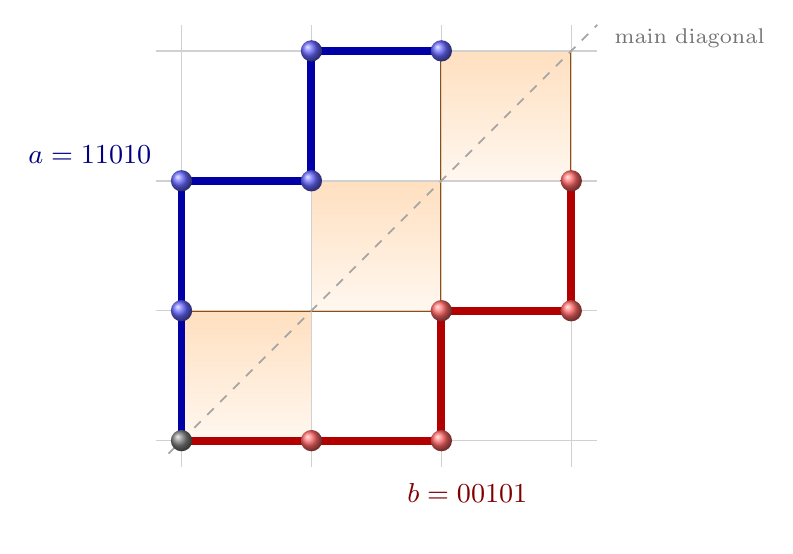
\includegraphics[width=0.62\textwidth]{fig_exceptional.png}
\caption{The exceptional pair of Lemma~\ref{lem:star} for $k=5$: $a=11010$ (upper path) and $b=00101$ (lower path). At every level from $1$ to $k$ the two paths are at different points, so they share no edge and $B_5(a,b)=0=k+1$ in $\F_2$. The shaded unit squares $Q_{(0,0)}$, $Q_{(1,1)}$ and $Q_{(2,2)}$ on the main diagonal separate the two paths: the path of $a$ passes above and to the left of them, the path of $b$ below and to the right.}
\label{fig:exceptional}
\end{figure}

For $p\in L(k)$ and $0\le\ell\le k$ let $\pi_p(\ell)=(\ell-\wt(p_{\le\ell}),\wt(p_{\le\ell}))$, where $p_{\le\ell}=p_1\cdots p_\ell$, be the point the path of $p$ reaches after $\ell$ steps. It is the only point of the path at level $\ell$. Let $V_p$ be the indicator function of the set of these points. For a lattice point $v=(x,y)$ let $Q_v$ be the unit square with lower left corner $v$, and let $\partial Q_v$ be the set of its four sides.

\begin{lemma}\label{lem:cell}
Let $p\in L(k)$ and let $v$ be a lattice point of level $\ell\le k-2$. Then
\[
|E(p)\cap\partial Q_v|=V_p(v)+V_p\bigl(v+(1,1)\bigr).
\]
If $c\in L(k)$ passes through $v$ and $v+(1,1)$ and $c'$ is obtained from $c$ by exchanging the letters in positions $\ell+1$ and $\ell+2$, then $B_k(p,c)+B_k(p,c')=V_p(v)+V_p(v+(1,1))$ in $\F_2$.
\end{lemma}

\begin{proof}
The bottom and left sides of $Q_v$ start at $v$. If the path of $p$ visits $v$, it leaves $v$ along exactly one of them, because $v$ has level $\ell<k$; otherwise it uses neither. The top and right sides end at $v+(1,1)$, and the path uses exactly one of them if it visits $v+(1,1)$ and neither otherwise. This proves the first identity. For the second, $c$ and $c'$ agree outside positions $\ell+1$ and $\ell+2$, where one of them reads $01$ and the other $10$; so their paths go around $Q_v$ on opposite sides and $E(c)$ and $E(c')$ differ exactly in $\partial Q_v$. Hence $|E(p)\cap E(c)|+|E(p)\cap E(c')|\equiv|E(p)\cap\partial Q_v|\pmod2$, and~\eqref{eq:common} finishes the proof.
\end{proof}

\begin{figure}[ht]
\centering
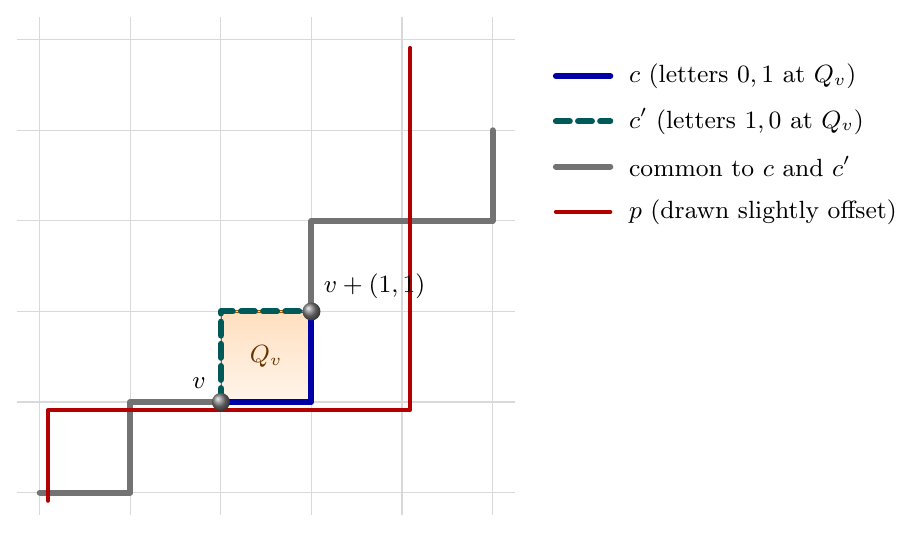
\includegraphics[width=0.62\textwidth]{cellflip.png}
\caption{Lemma~\ref{lem:cell}. The words $c$ and $c'$ differ in two consecutive letters, so their paths go around the square $Q_v$ on opposite sides and their edge sets differ by the four sides of $Q_v$. A path $p$ through $v$ uses one side at $v$ and, if it passes through $v+(1,1)$, one side there.}
\label{fig:cellflip}
\end{figure}

\begin{proof}[Proof of Lemma~\ref{lem:star}]
For $c\in L(k)$ put $f(c)=B_k(a,c)+B_k(b,c)$, so that $f(c)=0$ whenever $\wt(c)\notin\{\wt(a),\wt(b)\}$. For $e\in\{0,1\}$ and $p\in L(k)$ let $\lambda_e(p)$ be the length of the initial run of letters $e$ in $p$. The path of $0^k=0\cdots0$ runs along the $x$-axis, so it shares with the path of $p$ exactly the first $\lambda_0(p)$ edges; similarly for $1^k$. By~\eqref{eq:common},
\begin{equation}\label{eq:runs}
B_k(p,0^k)=\lambda_0(p),\qquad B_k(p,1^k)=\lambda_1(p)\qquad\text{in }\F_2 .
\end{equation}

\emph{Small $k$.} For $k=1$ the only pair is $a=1$, $b=0$, which is of the first kind with $u$ empty. For $k=2$ we need $B_2(a,b)=1$. If $\wt(b)=0$, then $b=00$ and $a\in\{01,10\}$, and $B_2(10,00)=0$, $B_2(01,00)=1$; so $(a,b)=(01,00)$. If $\wt(b)=1$, then $a=11$, and $B_2(11,01)=0$, $B_2(11,10)=1$; so $(a,b)=(11,10)$. Both are of the first kind. For $k=3$ we need $B_3(a,b)=0$, and the words $000$ and $111$ can serve as $c$ unless their weight is $\wt(a)$ or $\wt(b)$. If $\wt(b)=0$, then $b=000$ and $B_3(a,b)=\lambda_0(a)$ by~\eqref{eq:runs}, so $a\in\{100,001\}$; and $a=100$ fails at $c=111$, because $f(111)=\lambda_1(100)+\lambda_1(000)=1$. So $(a,b)=(001,000)$. The case $\wt(b)=2$ is symmetric under exchanging the letters $0$ and $1$ and the roles of $a$ and $b$;\footnote{Exchanging the letters reflects all paths in the diagonal, which preserves common edges; it turns a pair $(a,b)$ with $\wt(a)=\wt(b)+1$ into the pair $(\bar b,\bar a)$ with the same property.} it leaves $(a,b)=(111,110)$. If $\wt(b)=1$, both $000$ and $111$ are available, so $\lambda_0(a)\equiv\lambda_0(b)$ and $\lambda_1(a)\equiv\lambda_1(b)$. The pairs $(\lambda_0,\lambda_1)\bmod 2$ of $110,101,011$ are $(0,0),(0,1),(1,0)$ and those of $100,010,001$ are $(0,1),(1,0),(0,0)$, which leaves the pairs $(101,100)$, $(011,010)$ and $(110,001)$; all three have $B_3(a,b)=0$. The first two are of the first kind and the third is $1(10)^1,0(01)^1$.

From now on $k\ge4$. Let $J=V_a+V_b$ in $\F_2$. At each level $a$ and $b$ have one point each, so $J$ takes the value $1$ at exactly two points of a level where $a$ and $b$ are apart and vanishes on the levels where they meet; in particular $J(0,0)=0$.

\emph{Testable points.} Call a lattice point $v=(x,y)$ of level $\ell\le k-2$ \emph{testable} if some word $c$ of weight outside $\{\wt(a),\wt(b)\}$ passes through $v$ and $v+(1,1)$. For such $v$ the word $c'$ of Lemma~\ref{lem:cell} has the same weight as $c$, so $f(c)=f(c')=0$, and adding the identities of Lemma~\ref{lem:cell} for $p=a$ and $p=b$ gives
\begin{equation}\label{eq:diag}
J(v)=J\bigl(v+(1,1)\bigr)\qquad\text{for every testable }v .
\end{equation}
A word through $v$ and $v+(1,1)$ has $y+1$ letters $1$ among its first $\ell+2$ letters and $k-\ell-2$ further letters, so its weight can be any $t$ with $y+1\le t\le k-x-1$, an interval of $k-\ell-1$ integers. Since $\{\wt(a),\wt(b)\}=\{\wt(b),\wt(b)+1\}$ consists of two consecutive integers, we get:
\begin{enumerate}[label=\textup{(T\arabic*)}]
\item every point of level $\ell\le k-4$ is testable;
\item a point $(x,y)$ of level $k-3$ is testable unless $y=\wt(b)-1$.
\end{enumerate}
Indeed, for $\ell\le k-4$ the interval has at least three integers, and for $\ell=k-3$ it is $\{y+1,y+2\}$, which equals $\{\wt(b),\wt(b)+1\}$ exactly when $y=\wt(b)-1$.

\emph{Diagonals.} For $\ell\le k-2$ let $D_\ell$ be the set of differences $x-y$ over the points $(x,y)$ of level $\ell$ with $J(x,y)=1$. Then $D_\ell$ has $0$ or $2$ elements, all of the parity of $\ell$ and in $[-\ell,\ell]$, and $D_0=\varnothing$. For $\ell\le k-4$ and $|d|\le\ell$, the point of level $\ell+2$ with difference $d$ is $v+(1,1)$ for the point $v$ of level $\ell$ with difference $d$, so (T1) and~\eqref{eq:diag} give
\begin{equation}\label{eq:D}
D_{\ell+2}\cap[-\ell,\ell]=D_\ell\qquad(0\le\ell\le k-4).
\end{equation}
In particular $D_\ell\subseteq D_{\ell+2}$, and since both sets have at most two elements, $D_\ell\ne\varnothing$ implies $D_{\ell+2}=D_\ell$.

Suppose $\ell_0\le k-2$ is the smallest level of a given parity with $D_{\ell_0}\ne\varnothing$, and $\ell_0\ge2$. By~\eqref{eq:D}, $D_{\ell_0}\cap[-(\ell_0-2),\ell_0-2]=D_{\ell_0-2}=\varnothing$, so $D_{\ell_0}=\{\ell_0,-\ell_0\}$: the two paths are at $(\ell_0,0)$ and $(0,\ell_0)$, so one word begins with $\ell_0$ letters $0$ and the other with $\ell_0$ letters $1$, and the paths are apart at every level $1,\dots,\ell_0$. As $D_{\ell_0-2}=\varnothing$, the paths meet at level $\ell_0-2$, which is possible only for $\ell_0=2$; and then $D_1\ne\varnothing$. Applying this to both parities, we find three cases.
\begin{enumerate}[label=(\Roman*)]
\item $a_1=b_1$. Then $D_1=\varnothing$, so no odd level has $D_\ell\ne\varnothing$ (the smallest such level would be at least $3$), and no even level has $D_\ell\ne\varnothing$ (the smallest would be $2$, which needs $D_1\ne\varnothing$). So $D_\ell=\varnothing$ for all $\ell\le k-2$: the words $a$ and $b$ agree in their first $k-2$ letters.
\item $a_1\ne b_1$ and $D_\ell=\varnothing$ for every even $\ell\le k-2$. Then the paths are apart at level $1$ and meet at level $2$, necessarily at $(1,1)$: one word begins with $10$ and the other with $01$.
\item $a_1\ne b_1$ and $D_2\ne\varnothing$. Then $D_1=\{1,-1\}$ and $D_2=\{2,-2\}$, and by~\eqref{eq:D} $D_\ell=\{1,-1\}$ for odd $\ell\le k-2$ and $D_\ell=\{2,-2\}$ for even $2\le\ell\le k-2$.
\end{enumerate}

\emph{Case} (I). Let $t$ be the first position where $a$ and $b$ differ; then $t\in\{k-1,k\}$. If $t=k-1$, then the first $k-2$ positions count in $B_k(a,b)$, position $k-1$ does not, and position $k$ does not either, because $\wt(a_{<k})\ne\wt(b_{<k})$. So $B_k(a,b)=k-2=k$ in $\F_2$, contrary to the hypothesis $B_k(a,b)=k+1$. Hence $t=k$, and $\wt(a)=\wt(b)+1$ gives $a=u1$ and $b=u0$ with $u=a_{<k}$.

\emph{Case} (II). Both words contain a letter $1$ among their first two letters, so $\wt(a),\wt(b)\ge1$ and $c=0^k$ is admissible in the hypothesis. By~\eqref{eq:runs}, $f(0^k)=\lambda_0(a)+\lambda_0(b)=0+1=1$, a contradiction.

\emph{Case} (III), $k$ even. The paths are apart at every level from $1$ to $k-2$. At level $k-2$ their differences are $2$ and $-2$, so at level $k-1$ they are in $\{1,3\}$ and $\{-3,-1\}$, and the paths are apart there too. Hence no position $i\ge2$ counts in $B_k(a,b)$, and position $1$ does not count because $a_1\ne b_1$. So $B_k(a,b)=0$, while $k+1=1$ in $\F_2$, a contradiction.

\emph{Case} (III), $k=2j+1$ odd. Then $j\ge2$. Let $p^+$ be the one of $a,b$ whose path has difference $+2$ at level $2$, and $p^-$ the other. Following the differences $1,2,1,2,\dots$ level by level, $p^+$ is at $(i+1,i)$ at level $2i+1$ and at $(i+1,i-1)$ at level $2i$, for every level from $1$ to $k-2$; so its first $k-2$ letters are $0(01)^{j-1}$, and at levels $k-3$ and $k-2$ it is at $v^+=(j,j-2)$ and $(j,j-1)$. Symmetrically, $p^-$ begins with $1(10)^{j-1}$ and passes through $v^-=(j-2,j)$ and $(j-1,j)$. The points $v^+$ and $v^-$ have level $k-3$ and different second coordinates, so by (T2) at least one of them is testable.

If $v^+$ is testable, then~\eqref{eq:diag} gives $J(j+1,j-1)=J(v^+)=1$. The path of $p^-$ cannot reach $(j+1,j-1)$ from $(j-1,j)$, so $p^+$ passes through it, and the letter of $p^+$ in position $k-1$ is $0$; then $\wt(p^+)\le (j-1)+1=j$. If $v^-$ is testable, then in the same way $p^-$ passes through $(j-1,j+1)$ and $\wt(p^-)\ge j+1$.

If both are testable, the weights of $p^+$ and $p^-$ differ by $1$, so $\wt(p^+)=j$ and $\wt(p^-)=j+1$. Then $p^+=0(01)^{j-1}01=0(01)^j=b$ and $p^-=1(10)^{j-1}10=1(10)^j=a$, the exceptional pair.

If $v^+$ is not testable, then $j-2=\wt(b)-1$ by (T2), so $\wt(a)=j$ and $\wt(b)=j-1$; but $v^-$ is testable, so one of $a,b$ has weight at least $j+1$, a contradiction. If $v^-$ is not testable, then $j=\wt(b)-1$, so $\wt(b)=j+1$ and $\wt(a)=j+2$; but $v^+$ is testable, so one of $a,b$ has weight at most $j$, again a contradiction.
\end{proof}

\section{Groupings and the proof of Theorem~\ref{thm:B}}\label{sec:groupings}

\begin{proposition}\label{prop:groupings}
An admissible grouping of $L(k)$ either has no pairs, or its pairs are the pairs $(u1,u0)$ for all $u\in L(k-1)$ and it has no singletons.
\end{proposition}

The proof uses the following formula for the pairs that do occur.

\begin{lemma}\label{lem:canonical}
For $u\in L(k-1)$ and $c\in L(k)$,
\[
f_{u1,u0}(c)=\Iv{\wt(c_{<k})=\wt(u)} .
\]
\end{lemma}

\begin{proof}
By Lemma~\ref{lem:basic}(b), $B_k(ue,c)=B_{k-1}(u,c_{<k})+\Iv{e=c_k}\,\Iv{\wt(u)=\wt(c_{<k})}$. Adding the cases $e=1$ and $e=0$ gives the claim, since exactly one of them has $e=c_k$.
\end{proof}

\begin{proof}[Proof of Proposition~\ref{prop:groupings}]
Suppose the grouping has a pair. Every word of $L(k)$ belongs to some item, so for a pair $(a,b)$, (G2) gives $f_{a,b}(c)=0$ for all $c$ with $\wt(c)\notin\{\wt(a),\wt(b)\}$. Together with (G1), the pair satisfies the hypotheses of Lemma~\ref{lem:star}. So every pair is either \emph{canonical}, of the form $(u1,u0)$, or $k=2j+1\ge3$ and the pair is $(a^*,b^*)=(1(10)^j,0(01)^j)$.

\emph{The exceptional pair does not occur.} Suppose $(a^*,b^*)$ is a pair. Here $\wt(a^*)=j+1$, $\wt(b^*)=j$, the last letter of $a^*$ is $0$ and that of $b^*$ is $1$, so $\wt(a^*_{<k})=j+1$ and $\wt(b^*_{<k})=j-1$. Since $\binom{2j+1}{j}\ge3$, there is a word $c\ne b^*$ of weight $j$. By (G3) it is not a singleton, and it is not in the pair $(a^*,b^*)$, so it lies in a canonical pair $(u1,u0)$, with $\wt(u)=j-1$ if $c=u1$ and $\wt(u)=j$ if $c=u0$. This pair is not $(a^*,b^*)$, so neither $a^*$ nor $b^*$ belongs to it, and we may apply (G2) to the pair $(u1,u0)$ and the items $(a^*,0)$ and $(b^*,1)$. With Lemma~\ref{lem:canonical} this gives
\[
\Iv{\wt(u)=j+1}=f_{u1,u0}(a^*)=\Iv{\wt(a^*)=\wt(u1)}=\Iv{\wt(u)=j},
\]
\[
\Iv{\wt(u)=j-1}=f_{u1,u0}(b^*)=\Iv{\wt(b^*)=\wt(u0)}=\Iv{\wt(u)=j}.
\]
The first line excludes $\wt(u)=j$ and the second excludes $\wt(u)=j-1$, a contradiction.

\emph{All canonical pairs occur.} Now every pair is canonical. Let $\Lambda$ be the set of weights of the words that lie in pairs. By (G3), no singleton has a weight in $\Lambda$, so every word whose weight lies in $\Lambda$ is in a canonical pair. Let $t\in\Lambda$. If $t\ge1$, a word $v1$ of weight $t$ lies in a canonical pair, which must be $(v1,v0)$, so $t-1\in\Lambda$. If $t\le k-1$, a word $v0$ of weight $t$ lies in the pair $(v1,v0)$, so $t+1\in\Lambda$. As $\Lambda\ne\varnothing$, $\Lambda=\{0,1,\dots,k\}$. So there are no singletons, and each word $v0$ lies in a pair, which is $(v1,v0)$.
\end{proof}

\begin{theorem}\label{thm:main}
An admissible system of length $m$ is extremal if and only if it is a skeleton system $\Sigma(M,S)$ of a skeleton $(M,S)$ of $[m]$. Different skeletons of $[m]$ give different skeleton systems.
\end{theorem}

\begin{proof}
Skeleton systems are extremal by Proposition~\ref{prop:skeleton}, which also shows that different skeletons give different systems. We prove by induction on $m$ that every extremal admissible system $\cA$ of length $m$ is a skeleton system. For $m=0$, $L(0)$ consists of the empty word, so $\cA$ consists of one class containing it; this is $\Sigma(\varnothing,\varnothing)$.

Let $m\ge1$. By Proposition~\ref{prop:inequality} the system $\cG_0$ is extremal of length $m-1$, so by induction $\cG_0=\Sigma(M',S')$ for a skeleton $(M',S')$ of $[m-1]$; let $s_1<\dots<s_k$ be its free points. Lemma~\ref{lem:grouping} gives an admissible grouping of $L(k)$, and by Proposition~\ref{prop:groupings} there are two cases.

If the grouping has no pairs, the classes of $\cA$ are the sets $C_c0$ and $C_c1$ for $c\in L(k)$. Then $(M',S'\cup\{m\})$ is a skeleton of $[m]$, because the new free point $m$ lies under no arc, and its classes are exactly these sets. So $\cA=\Sigma(M',S'\cup\{m\})$.

Otherwise $k\ge1$ and the classes of $\cA$ are the sets $C_{u1}0\cup C_{u0}1$ for $u\in L(k-1)$. Such a set consists of the words $x\in L(m)$ with $x_p\ne x_q$ for the arcs $\{p,q\}$ of $M'$, with $x_{s_i}=u_i$ for $i<k$, and with $x_{s_k}\ne x_m$. Put $M=M'\cup\{\{s_k,m\}\}$ and $S=S'\setminus\{s_k\}$. Since $s_k$ is the last free point of $(M',S')$ and lies under no arc, every position between $s_k$ and $m$ belongs to an arc of $M'$ that lies entirely between them; so the new arc crosses no arc of $M'$, and it covers no free point. Thus $(M,S)$ is a skeleton of $[m]$ and $\cA=\Sigma(M,S)$.
\end{proof}

\begin{remark}\label{rem:growth}
The proof shows how extremal systems grow. Passing from length $m-1$ to length $m$ either adds a free point at the end, which doubles the number of classes and keeps their size, or turns the last free point into the left end of an arc that ends at $m$, which halves the number of classes and doubles their size. In both cases $\|\cA\|$ doubles.
\end{remark}

\section{Shankar's conjecture and the number of extremal systems}\label{sec:count}

\begin{proof}[Proof of Theorem~\ref{thm:A}]
Write the paths of $\cF$ as words in $L(2n)$. The collection $\{\cF\}$ is an admissible system of length $2n$: all words have weight $n$; for distinct $x,y\in\cF$ the number of common edges is even, so $B_{2n}(x,y)=0=2n$ in $\F_2$; and $B_{2n}(x,x)=2n=0$ by Lemma~\ref{lem:basic}(a). It has one class of size $2^n$, so it is extremal. By Theorem~\ref{thm:main} it equals $\Sigma(M,S)$ for a skeleton $(M,S)$ of $[2n]$. A skeleton system has $2^{|S|}$ classes, so $S=\varnothing$, $M$ is a noncrossing perfect matching of $[2n]$, and $\cF=C_\varnothing(M,\varnothing)=\cF_M$. Conversely each $\cF_M$ is such a family by Proposition~\ref{prop:skeleton}, and different matchings give different families. Hence there are exactly $C_n$ such families.
\end{proof}

\begin{proposition}\label{prop:count}
For every $m\ge0$ there are exactly $\binom{m}{\lfloor m/2\rfloor}$ skeletons of $[m]$, and hence exactly $\binom{m}{\lfloor m/2\rfloor}$ extremal admissible systems of length $m$.
\end{proposition}

\begin{proof}
By Theorem~\ref{thm:main} we must count the skeletons of $[m]$. Attach to a skeleton $(M,S)$ the sequence $\varepsilon\in\{1,-1\}^m$ with $\varepsilon_i=1$ if $i$ is a free point or the smaller end of an arc, and $\varepsilon_i=-1$ if $i$ is the larger end of an arc (Figure~\ref{fig:skeleton}). Every $-1$ is preceded by the $+1$ of its arc, so all partial sums of $\varepsilon$ are nonnegative.

Conversely, given $\varepsilon\in\{1,-1\}^m$ with nonnegative partial sums, read it from left to right and match each $-1$ with the last unmatched $+1$ before it, which exists because the partial sum before the $-1$ is positive. The matched pairs form a noncrossing set $M$ of arcs.\footnote{If $\{p,q\}$ and $\{p',q'\}$ were matched with $p<p'<q<q'$, then when $q$ is read, $p'$ is unmatched and later than $p$, so $q$ would have been matched with $p'$ or a later position, not with $p$.} Let $S$ be the set of positions of the $+1$'s that stay unmatched. If $s\in S$ were under an arc $\{p,q\}$, then $s$ would be unmatched and later than $p$ when $q$ is read, so $q$ would not be matched with $p$. Hence $(M,S)$ is a skeleton. When $\varepsilon$ comes from a skeleton, this matching recovers its arcs. Indeed, for an arc $\{p,q\}$ every position strictly between $p$ and $q$ belongs to an arc that lies strictly between them; by induction on $q-p$ these positions are matched among themselves, so $p$ is the last unmatched $+1$ when $q$ is read. So the two maps are inverse to each other.

It remains to count the sequences $\varepsilon\in\{1,-1\}^m$ with nonnegative partial sums. Those with total sum $h\ge0$ have $(m-h)/2$ entries $-1$. Those among them with a negative partial sum correspond bijectively to all sequences with total sum $-h-2$: change the signs of all entries after the first partial sum equal to $-1$.\footnote{This is the reflection principle of D.~Andr\'e; see~\cite{Kr,De}. The first partial sum equal to $-1$ is preserved by the reflection, so the map is an involution between the two sets.} So there are $\binom{m}{(m-h)/2}-\binom{m}{(m-h)/2-1}$ good sequences with sum $h$. Writing $h=m-2s$ and summing over $0\le s\le\lfloor m/2\rfloor$, the sum telescopes to $\binom{m}{\lfloor m/2\rfloor}$.
\end{proof}

For $m=2n$ the skeletons without free points are the noncrossing perfect matchings, which correspond to the sequences with total sum $0$; their number is $\binom{2n}{n}-\binom{2n}{n-1}=C_n$, in accordance with Theorem~\ref{thm:A}. Theorem~\ref{thm:B} is the combination of Theorem~\ref{thm:main} and Proposition~\ref{prop:count}.

\begin{remark}\label{rem:classsizes}
By Proposition~\ref{prop:skeleton}, the classes of an extremal system all have the same size $2^{|M|}$, and their number $2^{|S|}$ is a power of $2$ with $|S|\equiv m\pmod2$. So an admissible system with, for instance, two classes is never extremal, whatever the length. This rigidity is what separates the odd problem of Section~\ref{sec:rect} from the even one.
\end{remark}

\section{The binary rank of grid graphs}\label{sec:rank}

\subsection{Chebyshev-type polynomials over $\F_2$}

Define polynomials $f_s\in\F_2[x]$ by
\[
f_0=0,\qquad f_1=1,\qquad f_{s+1}=x f_s+f_{s-1}\quad(s\ge1).
\]
Thus $f_2=x$, $f_3=x^2+1$, $f_4=x^3$, $f_5=x^4+x^2+1$, and $f_s$ is monic of degree $s-1$ for $s\ge1$. Over the integers these are, up to signs, the Chebyshev polynomials of the second kind evaluated at $x/2$, and over $\F_2$ they are the Fibonacci polynomials reduced modulo $2$~\cite{HL,Sutner00}.

\begin{lemma}\label{lem:fib}
\textup{(a)} For $s\ge1$, with $T=\begin{pmatrix}x&1\\1&0\end{pmatrix}$,
\[
T^s=\begin{pmatrix}f_{s+1}&f_s\\ f_s&f_{s-1}\end{pmatrix}.
\]
\textup{(b)} $f_{s+1}f_{s-1}+f_s^2=1$ for $s\ge1$; in particular $\gcd(f_s,f_{s+1})=1$.

\textup{(c)} $f_{p+q}=f_{p+1}f_q+f_pf_{q-1}$ for $p\ge0$ and $q\ge1$.

\textup{(d)} $\gcd(f_i,f_j)=f_{\gcd(i,j)}$ for all $i,j\ge0$, where $\gcd(i,0)=i$.
\end{lemma}

\begin{proof}
(a) For $s=1$ this is the definition of $T$, since $f_2=x$, $f_1=1$, $f_0=0$. If it holds for $s$, then multiplying by $T$ on the right gives the first column $(xf_{s+1}+f_s,\ xf_s+f_{s-1})=(f_{s+2},f_{s+1})$ and the second column $(f_{s+1},f_s)$.

(b) Take determinants in (a): $\det T=-1=1$ in $\F_2$, so $f_{s+1}f_{s-1}-f_s^2=1$, which is the claim since $-1=1$. A common divisor of $f_s$ and $f_{s+1}$ divides $1$.

(c) For $p=0$ the identity reads $f_q=f_1f_q+f_0f_{q-1}$, which holds. For $p\ge1$ compare the upper right entries of $T^{p+q}=T^pT^q$: the entry of the product is $f_{p+1}f_q+f_pf_{q-1}$.

(d) We may assume $i>j\ge1$, the cases $j=0$ and $i=j$ being trivial. By (c) with $p=i-j$ and $q=j$,
\[
\gcd(f_i,f_j)=\gcd(f_{i-j+1}f_j+f_{i-j}f_{j-1},\,f_j)=\gcd(f_{i-j}f_{j-1},\,f_j)=\gcd(f_{i-j},f_j),
\]
where the last step uses $\gcd(f_{j-1},f_j)=1$ from (b). So $\gcd(f_i,f_j)$ is unchanged when $i$ is replaced by $i-j$, and the Euclidean algorithm on the indices ends at $\gcd(f_{\gcd(i,j)},f_0)=f_{\gcd(i,j)}$.
\end{proof}

\subsection{The path and the grid}

Let $P_a$ be the adjacency matrix of the path with $a$ vertices, the $a\times a$ matrix over $\F_2$ with ones exactly in the positions $(i,i\pm1)$.

\begin{lemma}\label{lem:pathmatrix}
The characteristic polynomial of $P_a$ is $f_{a+1}$, and $P_a$ is cyclic: the vectors $e_1,P_ae_1,\dots,P_a^{a-1}e_1$ form a basis of $\F_2^a$. Consequently, for every $g\in\F_2[x]$,
\[
\dim\ker g(P_a)=\deg\gcd(g,f_{a+1}).
\]
\end{lemma}

\begin{proof}
Let $\chi_a=\det(xI+P_a)$, which over $\F_2$ is the characteristic polynomial. Expanding along the last row gives $\chi_a=x\chi_{a-1}+\chi_{a-2}$ (in characteristic two the sign of the second term disappears), with $\chi_0=1=f_1$ and $\chi_1=x=f_2$; so $\chi_a=f_{a+1}$. The vector $P_a^ke_1$ has its last nonzero coordinate in position $k+1$, because $P_a$ moves the support of a vector at most one step to the right and the coordinate $k+1$ of $P_a^ke_1$ counts the single path $1\to2\to\dots\to k+1$; so $e_1,\dots,P_a^{a-1}e_1$ are linearly independent. Hence $\F_2^a$ is a cyclic $\F_2[x]$-module with $x$ acting as $P_a$, isomorphic to $\F_2[x]/(f_{a+1})$, since the minimal polynomial of a cyclic matrix equals its characteristic polynomial. The kernel of multiplication by $g$ on $\F_2[x]/(h)$ is $(h/d)\,\F_2[x]/(h)$ with $d=\gcd(g,h)$, a module isomorphic to $\F_2[x]/(d)$, of dimension $\deg d$. For background on cyclic matrices see~\cite[Section~3.3]{HJ}.
\end{proof}

\begin{proof}[Proof of Theorem~\ref{thm:C}]
Index the vertices of $P_a\,\square\,P_b$ by pairs $(i,j)$ with $1\le i\le a$ and $1\le j\le b$, and write a vector $z\in\F_2^{ab}$ as the sequence of its rows $r_1,\dots,r_b\in\F_2^a$, where $r_j$ collects the coordinates $(i,j)$. The neighbours of $(i,j)$ are $(i\pm1,j)$ and $(i,j\pm1)$, so with the convention $r_0=r_{b+1}=0$ the equation $A_{a,b}z=0$ says
\[
P_ar_j+r_{j-1}+r_{j+1}=0\qquad(1\le j\le b).
\]
Equivalently $r_{j+1}=P_ar_j+r_{j-1}$ for $1\le j\le b$, so by induction $r_j=f_j(P_a)r_1$ for $0\le j\le b+1$, and the last equation is $f_{b+1}(P_a)r_1=r_{b+1}=0$. Conversely, every $r_1$ with $f_{b+1}(P_a)r_1=0$ determines a vector in the kernel by $r_j=f_j(P_a)r_1$. So $\ker A_{a,b}\cong\ker f_{b+1}(P_a)$, and by Lemmas~\ref{lem:pathmatrix} and~\ref{lem:fib}(d),
\[
\dim\ker A_{a,b}=\deg\gcd(f_{b+1},f_{a+1})=\deg f_{\gcd(a+1,b+1)}=\gcd(a+1,b+1)-1 .
\]
The rank is $ab$ minus this number.
\end{proof}

\begin{corollary}\label{cor:invertible}
$A_{a,b}$ is invertible over $\F_2$ if and only if $a+1$ and $b+1$ are coprime. The kernel of $A_{n,n}$ has dimension $n$, and every vector of it is determined by its first row.
\end{corollary}

Figure~\ref{fig:rank} shows the nullity $\gcd(a+1,b+1)-1$ for $a,b\le 24$. Note that $\rank A_{a,b}$ is always even, as it must be: a symmetric matrix with zero diagonal over $\F_2$ is the matrix of an alternating form, and alternating forms have even rank.

\begin{figure}[ht]
\centering
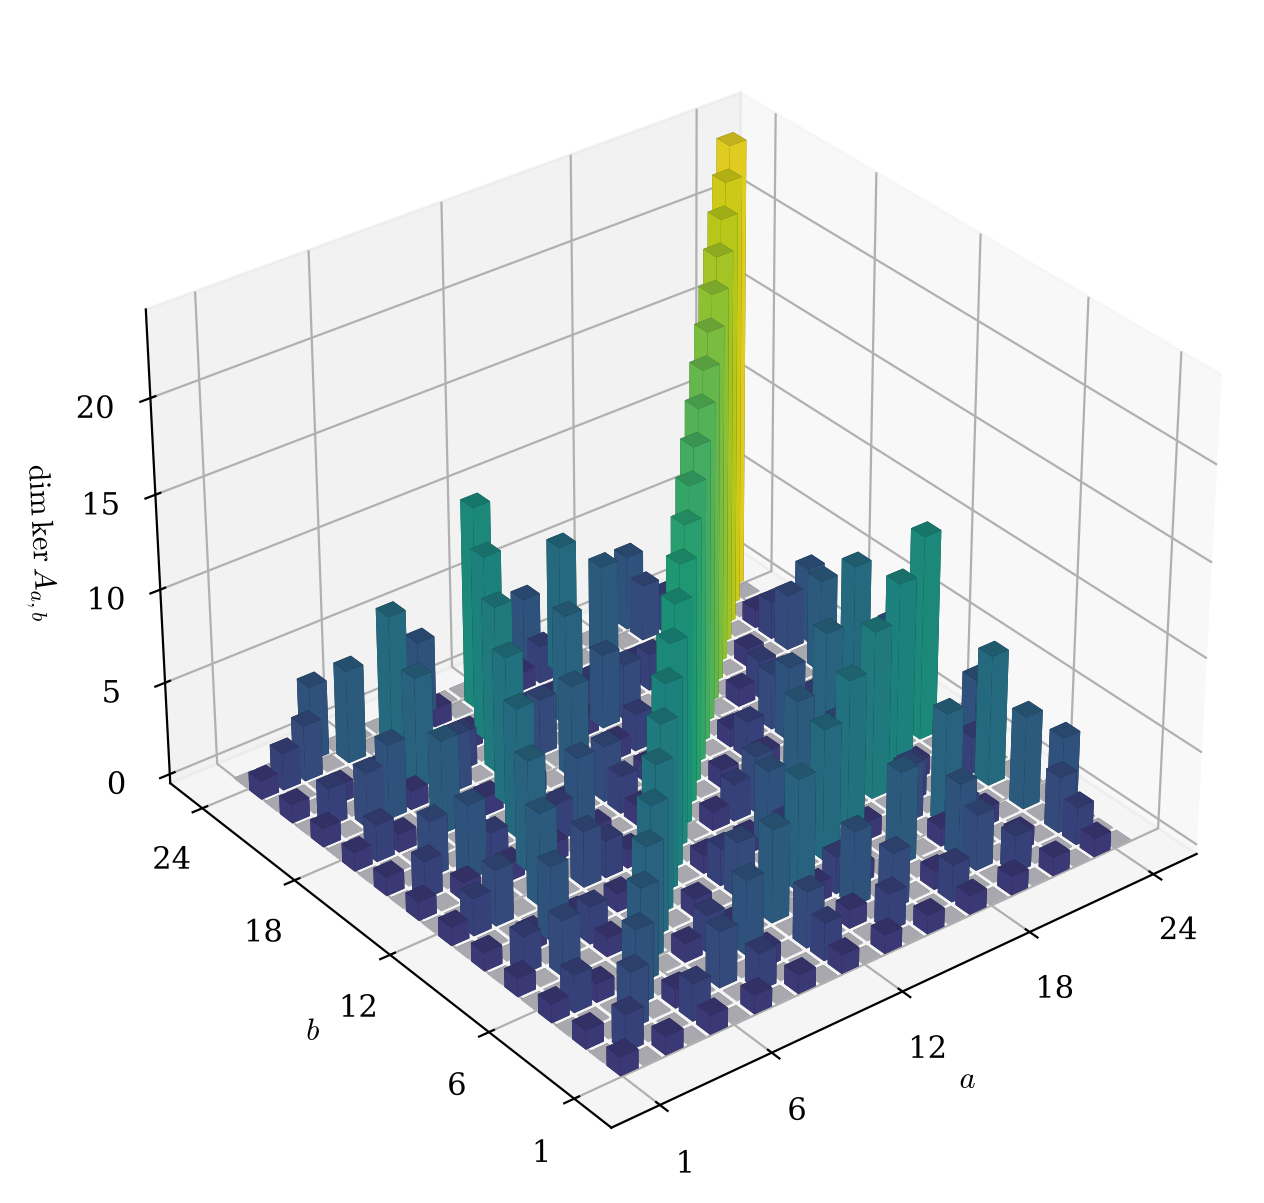
\includegraphics[width=0.82\textwidth]{fig_rank.png}
\caption{The nullity $\dim\ker A_{a,b}=\gcd(a+1,b+1)-1$ of the adjacency matrix of the $a\times b$ grid over $\F_2$, for $1\le a,b\le 24$. The diagonal $a=b$ carries the values $n$ found by Shankar; off the diagonal the nullity vanishes whenever $a+1$ and $b+1$ are coprime.}
\label{fig:rank}
\end{figure}

\section{Rectangles, both parities, and odd lengths}\label{sec:rect}

\subsection{Parity of the length decides the order of magnitude}

Fix $a,b\ge1$ and $m=a+b$. A family of paths from $(0,0)$ to $(a,b)$ is \emph{even} or \emph{odd} if every two distinct members share an even or an odd number of edges. In terms of words, an even family is a set of words of length $m$ and weight $b$ with $B_m(x,y)=0$ for $x\ne y$, and an odd family has $B_m(x,y)=1$ for $x\ne y$.

\begin{lemma}\label{lem:oneclass}
A set $\cF$ of words of length $m$ and weight $b$ is a one-class admissible system if and only if it is an even family and $m$ is even, or an odd family and $m$ is odd.
\end{lemma}

\begin{proof}
Conditions (A1) and (A3) hold for one class of words of one weight, and (A2) asks for $B_m(x,y)=m$ in $\F_2$ for all $x,y\in\cF$; for $x=y$ this always holds by Lemma~\ref{lem:basic}(a).
\end{proof}

\begin{proof}[Proof of Theorem~\ref{thm:D}, \textup{(i)} and \textup{(ii)}, exponential parts]
By the symmetry $x\mapsto\bar x$, which exchanges the letters and reflects paths in the diagonal, we may assume $a\ge b$. Let $M$ consist of the arcs $\{2i-1,2i\}$ for $1\le i\le b$, and let the remaining $a-b$ positions be free; free points after all arcs lie under no arc, so this is a skeleton of $[m]$. Its class $C_{0^{a-b}}$ consists of $2^b$ words of weight $b$, and by Proposition~\ref{prop:skeleton} any two of them have $B_m=B_{a-b}(0^{a-b},0^{a-b})=a-b$. If $m$ is even, then $a-b$ is even and the class is an even family; if $m$ is odd, it is an odd family. This proves the lower bounds $2^{\min(a,b)}$.

For the upper bounds, an even family with $m$ even, or an odd family with $m$ odd, is a one-class admissible system by Lemma~\ref{lem:oneclass}, so $|\cF|^2\le 2^m$ by Proposition~\ref{prop:inequality}. If $m$ is odd, $2^m$ is not a square, so $|\cF|<2^{m/2}$. If $m$ is even and $|\cF|=2^{m/2}$, the system $\{\cF\}$ is extremal, so by Theorem~\ref{thm:main} it is a skeleton system with one class; then $S=\varnothing$ and its words have weight $|M|=m/2$, so $b=m/2$ and $a=b$. Conversely $\Meven(n,n)=2^n$ by Theorem~\ref{thm:A}.
\end{proof}

\subsection{The Gram matrix of the path space}

The polynomial bounds rest on the edge space of the grid. Let $\Gamma_{a,b}$ be the grid graph with vertex set $\{0,\dots,a\}\times\{0,\dots,b\}$ and let $\langle\,,\rangle$ be the standard bilinear form on $\F_2^{E(\Gamma_{a,b})}$. Identify a path with the indicator vector of its edges, so that $\langle F,G\rangle=|E(F)\cap E(G)|\bmod2$. Let $W$ be the span of all paths from $(0,0)$ to $(a,b)$. For $1\le i\le a$ and $1\le j\le b$ let $c_{i,j}$ be the boundary of the unit square with lower left corner $(i-1,j-1)$, and let $Q=N^bE^a$ be the path along the left and top sides of the rectangle. This basis is Shankar's for $a=b$~\cite{Sh}.

\begin{lemma}\label{lem:basis}
The vectors $Q$ and $c_{i,j}$ $(1\le i\le a,\ 1\le j\le b)$ form a basis of $W$, which has dimension $ab+1$. In this basis the Gram matrix of $\langle\,,\rangle$ is
\[
G_W=\begin{pmatrix}m\bmod 2&q^{T}\\ q&A_{a,b}\end{pmatrix},\qquad q_{i,j}=\Iv{i=1}+\Iv{j=b}\in\F_2,
\]
where the cells are ordered as the vertices of $P_a\,\square\,P_b$.
\end{lemma}

\begin{proof}
Let $Z$ be the cycle space of $\Gamma_{a,b}$, the set of edge sets in which every vertex has even degree. It has dimension\footnote{A spanning tree of a connected graph has $|V|-1$ edges, and each of the remaining $|E|-|V|+1$ edges closes exactly one cycle with the tree. These fundamental cycles are linearly independent, since each contains an edge that no other contains, and every element of the cycle space is the sum of the fundamental cycles of its edges outside the tree; so they form a basis.} $|E|-|V|+1=a(b+1)+b(a+1)-(a+1)(b+1)+1=ab$, since $\Gamma_{a,b}$ is connected. The $ab$ cell boundaries are linearly independent: in a nonempty set of cells, take one with the largest $j$ and, among those, the largest $i$; its top side belongs to no other cell of the set, so the sum of the boundaries is not zero. Hence the cell boundaries form a basis of $Z$.

The sum of two paths from $(0,0)$ to $(a,b)$ lies in $Z$, because each interior vertex of a path has degree $2$ and the two endpoints have degree $1$ in each path. Every cell boundary is the sum of two paths: a path through $(i-1,j-1)$ that continues $EN$ and the same path continued $NE$. So $W=\F_2Q+Z$, and $Q\notin Z$ because $(0,0)$ has degree $1$ in $Q$. This gives the basis and the dimension.

Two distinct cell boundaries share one edge if the cells are adjacent and none otherwise, and a cell boundary has four edges; so the lower right block is $A_{a,b}$. The path $Q$ contains the whole left side and the whole top side of the rectangle and no other edge. The boundary $c_{i,j}$ meets the left side exactly when $i=1$, in one edge, and the top side exactly when $j=b$, in one edge. This gives $q$. Finally $\langle Q,Q\rangle=|Q|=m$ modulo $2$.
\end{proof}

\begin{proposition}\label{prop:gram}
Let $r=\rank A_{a,b}=ab-\gcd(a+1,b+1)+1$.
\begin{enumerate}[label=\textup{(\alph*)}]
\item $\rank G_W\le r+2$.
\item If $m$ is even, then $\rank G_W=r$ if $q$ lies in the column space of $A_{a,b}$, and $\rank G_W=r+2$ otherwise.
\item If $a=b$, then $q=A_{n,n}u$ for the vector $u_{i,j}=\Iv{i<j}$, so $\rank G_W=n(n-1)$.
\end{enumerate}
\end{proposition}

\begin{proof}
(a) Bordering a matrix by one row and one column raises the rank by at most $2$.

(b) If $m$ is even, every basis vector of $W$ has an even number of edges, and $x\mapsto\langle x,x\rangle=|x|\bmod 2$ is linear, so $\langle x,x\rangle=0$ on $W$: the form is alternating and its rank is even. If $q=A_{a,b}u$, put $Q'=Q+\sum u_{i,j}c_{i,j}$. Then $\langle Q',c_{i,j}\rangle=q_{i,j}+(A_{a,b}u)_{i,j}=0$ and $\langle Q',Q'\rangle=0$, so in the basis $Q',c_{i,j}$ the Gram matrix is $0\oplus A_{a,b}$, of rank $r$. If $q$ is not in the column space, then the rank of the matrix $(q\mid A_{a,b})$ is $r+1$, so $\rank G_W\ge r+1$, and being even and at most $r+2$, it equals $r+2$.

(c) We check $(A_{n,n}u)_{i,j}=q_{i,j}$ cell by cell; the four possible neighbours of $(i,j)$ are $(i\pm1,j)$ and $(i,j\pm1)$, and a neighbour contributes when it exists and lies strictly above the diagonal. If $i\le j$, the neighbours $(i-1,j)$ and $(i,j+1)$ lie above the diagonal whenever they exist, that is when $i\ge2$ and when $j\le n-1$; the neighbours $(i+1,j)$ and $(i,j-1)$ lie above the diagonal either both (when $i\le j-2$) or neither (when $i\in\{j-1,j\}$). So $(A_{n,n}u)_{i,j}=\Iv{i\ge2}+\Iv{j\le n-1}=\Iv{i=1}+\Iv{j=n}=q_{i,j}$. If $i\ge j+1$, no neighbour lies above the diagonal, so $(A_{n,n}u)_{i,j}=0$; and $q_{i,j}=0$ because $i\ne1$ and $j\le n-1$. By (b) and Theorem~\ref{thm:C}, $\rank G_W=n^2-n$.
\end{proof}

Write $\delta(a,b)=0$ if $q$ lies in the column space of $A_{a,b}$ and $\delta(a,b)=1$ otherwise. Table~\ref{tab:delta} in Appendix~\ref{app:comp} lists $\delta$ for $a,b\le10$; for instance $\delta(1,3)=1$ and $\delta(2,4)=0$.

\begin{proof}[Proof of Theorem~\ref{thm:D}, \textup{(i)} and \textup{(ii)}, polynomial parts]
Let $\cF=\{F_1,\dots,F_N\}$ be a family and $H=(\langle F_s,F_t\rangle)_{s,t}$ its Gram matrix. Writing each $F_s$ in the basis of Lemma~\ref{lem:basis} as the column $X_s$ of a matrix $X$, we have $H=X^TG_WX$, so $\rank H\le\rank G_W$.

If $m$ is even and $\cF$ is odd, then $H=J+I$, where $J$ is the all-ones matrix of size $N$, since the diagonal entries are $m\bmod2=0$. Over $\F_2$, $(J+I)^2=NJ+I$; so $J+I$ is invertible when $N$ is even, and when $N$ is odd its leading principal submatrix of size $N-1$ is invertible.\footnote{That submatrix is $J'+I$, where $J'$ is the all-ones matrix of the even size $N-1$. The same computation gives $(J'+I)^2=(N-1)J'+I=I$, so $J'+I$ is its own inverse. For even $N$ the identity reads $(J+I)^2=I$ directly.} In both cases $\rank H\ge N-1$, so $N\le\rank G_W+1\le r+3$ by Proposition~\ref{prop:gram}(a). More precisely $N\le r+2\delta(a,b)+1$.

If $m$ is odd and $\cF$ is even, then $H=I$, so $N=\rank H\le\rank G_W\le r+2$.
\end{proof}

For $a=b=n$ the bound reads $\Modd(n,n)\le n(n-1)+1$, which is Shankar's theorem; Figure~\ref{fig:gram} shows the vector $u$ of Proposition~\ref{prop:gram}(c).

\begin{figure}[ht]
\centering
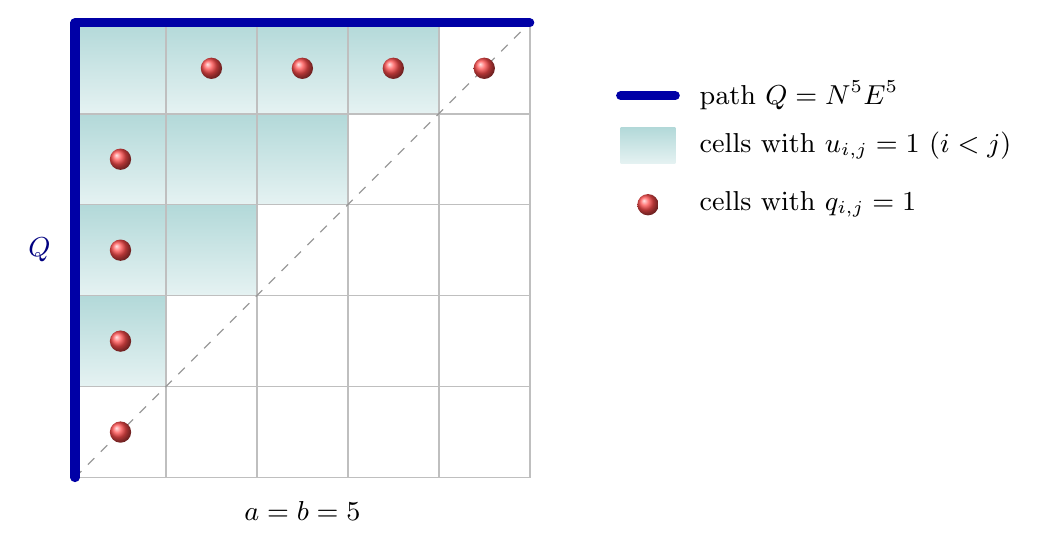
\includegraphics[width=0.66\textwidth]{fig_gram.png}
\caption{The basis of Lemma~\ref{lem:basis} for $a=b=5$. The path $Q=N^5E^5$ runs along the left and top sides. The cells with $q_{i,j}=1$ carry a dot; the shaded cells, strictly above the diagonal, form the vector $u$ with $A_{5,5}u=q$. Replacing $Q$ by $Q+\sum_{i<j}c_{i,j}$ makes it orthogonal to every cell.}
\label{fig:gram}
\end{figure}

\subsection{Changing the parity by one step}

\begin{proof}[Proof of Theorem~\ref{thm:D}, \textup{(iii)}]
Let $\cF$ be a family of paths from $(0,0)$ to $(a,b)$ and $e\in\{0,1\}$. All words of $\cF$ have weight $b$, so Lemma~\ref{lem:basic}(b) gives $B_{m+1}(xe,ye)=B_m(x,y)+1$ for all $x,y\in\cF$. Hence $\cF e$ is odd if $\cF$ is even and even if $\cF$ is odd. For $e=0$ the new paths end at $(a+1,b)$, for $e=1$ at $(a,b+1)$.
\end{proof}

In particular $\Modd(n+1,n)\ge\Meven(n,n)=2^n$, $\Modd(n,n)\ge\Meven(n,n-1)$ and $\Meven(n+1,n)\ge\Modd(n,n)$. The exhaustive computations of Appendix~\ref{app:comp} show that
\begin{equation}\label{eq:transferobs}
\Modd(n,n)=\Meven(n,n-1)\qquad(2\le n\le 6),
\end{equation}
so that for these $n$ an optimal odd family of the square may be taken to end with a north step.

\subsection{One row of cells}

For $b=1$ the problem can be solved completely, and the answer shows both orders of magnitude at once.

\begin{proposition}\label{prop:onerow}
Let $a\ge1$ and $p\in\{0,1\}$, and let $M_p(a,1)$ be $\Meven(a,1)$ for $p=0$ and $\Modd(a,1)$ for $p=1$. Then
\[
M_p(a,1)=\begin{cases}\lfloor a/2\rfloor+1,& a+p\ \text{even},\\ 2,& a+p\ \text{odd}.\end{cases}
\]
\end{proposition}

\begin{proof}
The paths from $(0,0)$ to $(a,1)$ are $F_i=E^iNE^{a-i}$ for $0\le i\le a$. For $i<j$, the paths $F_i$ and $F_j$ share the first $i$ edges of the bottom row and the last $a-j$ edges of the top row, and nothing else; so $|E(F_i)\cap E(F_j)|=i+a-j\equiv i+j+a\pmod2$. A family $\{F_i:i\in X\}$ therefore has the required parity if and only if $i+j\equiv a+p$ for all distinct $i,j\in X$.

If $|X|\ge3$, take distinct $i,j,k\in X$; from $i+j\equiv i+k\equiv j+k$ we get $i\equiv j\equiv k$, so all elements of $X$ have one parity, and then $a+p\equiv 2i\equiv0$. If $|X|=2$, the condition says that the two indices have the parity relation dictated by $a+p$.

If $a+p$ is even, the admissible families are the sets of indices of one parity, and the largest has $\lfloor a/2\rfloor+1$ elements (the even indices $0,2,\dots$). If $a+p$ is odd, no three indices are allowed, and any two indices of opposite parity are, for instance $\{0,1\}$; so the maximum is $2$.
\end{proof}

When $m=a+1$ has the parity $p$ of the intersections, Theorem~\ref{thm:D} gives $2\le M_p(a,1)<2^{(a+1)/2}$, and indeed the answer is $2$; when the parities differ, the answer grows linearly, in accordance with the polynomial bounds.

\subsection{Two rows of cells}

For $b=2$ the largest families grow linearly in $a$ for both parities, and the parity that Theorem~\ref{thm:D} bounds by a polynomial gives the larger families. A path from $(0,0)$ to $(a,2)$ is $E^iNE^{i'-i}NE^{a-i'}$ for a unique pair $0\le i\le i'\le a$, its two north steps lying on the lines $x=i$ and $x=i'$; we write it as $(i,i')$.

\begin{lemma}\label{lem:tworows}
Let $p=(i,i')$ and $q=(k,k')$ be paths from $(0,0)$ to $(a,2)$, ordered so that $i<k$, or $i=k$ and $i'\le k'$, and put $d(p,q)=|E(p)\cap E(q)|-a$. Then, modulo $2$,
\begin{enumerate}[label=\textup{(\Alph*)}]
\item $d(p,q)\equiv i+k'$ if $i'<k$;
\item $d(p,q)\equiv i+k'+\Iv{i=i'}+\Iv{k=k'}$ if $i'=k$;
\item $d(p,q)\equiv i+i'+k+k'+\Iv{i=k}+\Iv{i'=k'}$ if $k<i'$.
\end{enumerate}
\end{lemma}

\begin{proof}
The path $p$ uses the edges $[x,x+1]\times\{0\}$ for $x<i$, $[x,x+1]\times\{1\}$ for $i\le x<i'$ and $[x,x+1]\times\{2\}$ for $x\ge i'$, together with the vertical edges $\{i\}\times[0,1]$ and $\{i'\}\times[1,2]$. Comparing with $q$ row by row,
\[
|E(p)\cap E(q)|=\min(i,k)+\max\bigl(0,\min(i',k')-\max(i,k)\bigr)+a-\max(i',k')+\Iv{i=k}+\Iv{i'=k'} .
\]
In case (A) we have $i\le i'<k\le k'$, so the four terms are $i$, $0$, $a-k'$ and $0$, $0$. In case (B) the middle term is $\max(0,i'-k)=0$, the third is $a-k'$, and $\Iv{i=k}=\Iv{i=i'}$, $\Iv{i'=k'}=\Iv{k=k'}$ because $k=i'$. In case (C) the middle term is $\min(i',k')-k\ge0$, and $\min(i',k')-\max(i',k')\equiv i'+k'$.
\end{proof}

A family of paths from $(0,0)$ to $(a,2)$ is even exactly when $d\equiv a$ on all pairs and odd exactly when $d\equiv a+1$. The length $a+2$ has the parity of $a$, so the one-class case of Lemma~\ref{lem:oneclass} is $d\equiv0$, and the other case is $d\equiv1$.

\begin{theorem}\label{thm:tworows}
Let $a\ge2$.
\begin{enumerate}[label=\textup{(\roman*)}]
\item If $a$ is even, then $\Meven(a,2)\ge\lfloor a/2\rfloor+3$ and $\Modd(a,2)\ge\lfloor(5a-2)/4\rfloor$.
\item If $a$ is odd, then $\Modd(a,2)\ge\lfloor a/2\rfloor+3$ and $\Meven(a,2)\ge\lfloor(5a-1)/4\rfloor$.
\end{enumerate}
\end{theorem}

\begin{proof}
\emph{The one-class case, $d\equiv0$.} Let $e=2\lfloor a/2\rfloor$ be the largest even number at most $a$, and let $\cF$ consist of the paths $D_k=(k,k)$ for even $0\le k\le a$, together with $(0,1)$ and $(e-1,e)$. These are $\lfloor a/2\rfloor+3$ distinct paths, since $e\ge2$. Two paths $D_k$, $D_l$ with $k<l$ fall under (A), with $d\equiv k+l\equiv0$. The path $(0,1)$ meets $D_0$ under (B), with $D_0$ first, and $d\equiv0+1+1+0\equiv0$, and it meets $D_k$ with $k\ge2$ under (A) with $d\equiv0+k\equiv0$. The path $(e-1,e)$ meets $D_e$ under (B) with $d\equiv(e-1)+e+0+1\equiv0$, and meets $D_k$ with $k\le e-2$ under (A), now with $D_k$ first, so that $d\equiv k+e\equiv0$. Finally, if $e\ge4$ the paths $(0,1)$ and $(e-1,e)$ fall under (A) with $d\equiv0+e\equiv0$, and if $e=2$ they fall under (B) with $d\equiv0+2\equiv0$.

\emph{The case $d\equiv1$ for odd $a$.} Let $\cF$ consist of
\[
\begin{gathered}
P_j=(2j,2j+1)\ \ (0\le 2j\le a-3),\qquad Q_t=(4t,4t+3)\ \ (0\le 4t\le a-5),\\
R_o=(o,a)\ \ (o\ \text{odd},\ 1\le o\le a),
\end{gathered}
\]
which are $\frac{a-1}2+\lfloor\frac{a-1}4\rfloor+\frac{a+1}2=a+\lfloor\frac{a-1}4\rfloor=\lfloor\frac{5a-1}4\rfloor$ distinct paths. We go through the pairs.
\begin{itemize}
\item $P_j,P_l$ with $j<l$: case (A), $d\equiv 2j+2l+1\equiv1$. Likewise $Q_t,Q_u$ with $t<u$: case (A), $d\equiv4t+4u+3\equiv1$.
\item $R_o,R_{o'}$ with $o<o'<a$: case (C), $d\equiv o+a+o'+a+0+1\equiv1$. With $o'=a$: case (B), $d\equiv o+a+0+1\equiv1$.
\item $P_j$ and $R_o$: if $o\ge2j+3$, case (A) with $P_j$ first, $d\equiv2j+a\equiv1$; if $o=2j+1$, case (B), $d\equiv2j+a\equiv1$, since $2j+1\le a-2$ means that neither path is of the form $(k,k)$; if $o\le2j-1$, case (C) with $R_o$ first, $d\equiv o+a+2j+(2j+1)\equiv1$.
\item $P_j$ and $Q_t$: the left end $2j$ of $P_j$ is even and its right end is odd. If $2j+1<4t$ or $2j\ge4t+4$, case (A) gives $d\equiv1$, since the left end of the first path is even and the right end of the second is odd. If $2j=4t$, case (C) with $P_j$ first and equal left ends gives $d\equiv 4t+(4t+1)+4t+(4t+3)+1\equiv1$. If $2j=4t+2$, case (C) with $Q_t$ first and equal right ends gives $d\equiv4t+(4t+3)+(4t+2)+(4t+3)+1\equiv1$.
\item $Q_t$ and $R_o$, where $4t+3\le a-2$: if $o\ge4t+5$, case (A), $d\equiv4t+a\equiv1$; if $o=4t+3$, case (B), $d\equiv 4t+a\equiv1$; if $o=4t+1$, case (C) with $Q_t$ first, $d\equiv4t+(4t+3)+(4t+1)+a\equiv1$; if $o\le4t-1$, case (C) with $R_o$ first, $d\equiv o+a+4t+(4t+3)\equiv1$.
\end{itemize}

\emph{The case $d\equiv1$ for even $a$.} Each rule of the lemma is a sum of an even number of endpoints and of indicators of coincidences between endpoints, so the rules, and the case into which a pair falls, are unchanged when every endpoint is increased by $1$. Shifting the family just constructed for the odd number $a-1$ by one unit to the right therefore gives paths $(2j+1,2j+2)$, $(4t+1,4t+4)$ and $(o+1,a)$ from $(0,0)$ to $(a,2)$ with $d\equiv1$ on all pairs. Add the path $(0,a)$. It meets a path $(k,k')$ with $1\le k<a$ under (C), with $d\equiv a+k+k'+\Iv{k'=a}\equiv k+k'+\Iv{k'=a}$, which is $1$ for $(2j+1,2j+2)$ and $(4t+1,4t+4)$ (an odd sum, $k'<a$) and for $(o+1,a)$ with $o+1<a$ (an even sum, $k'=a$); and it meets $(a,a)$ under (B) with $d\equiv a+0+1\equiv1$. The family has $\lfloor(5(a-1)-1)/4\rfloor+1=\lfloor(5a-2)/4\rfloor$ members.
\end{proof}

\begin{figure}[ht]
\centering
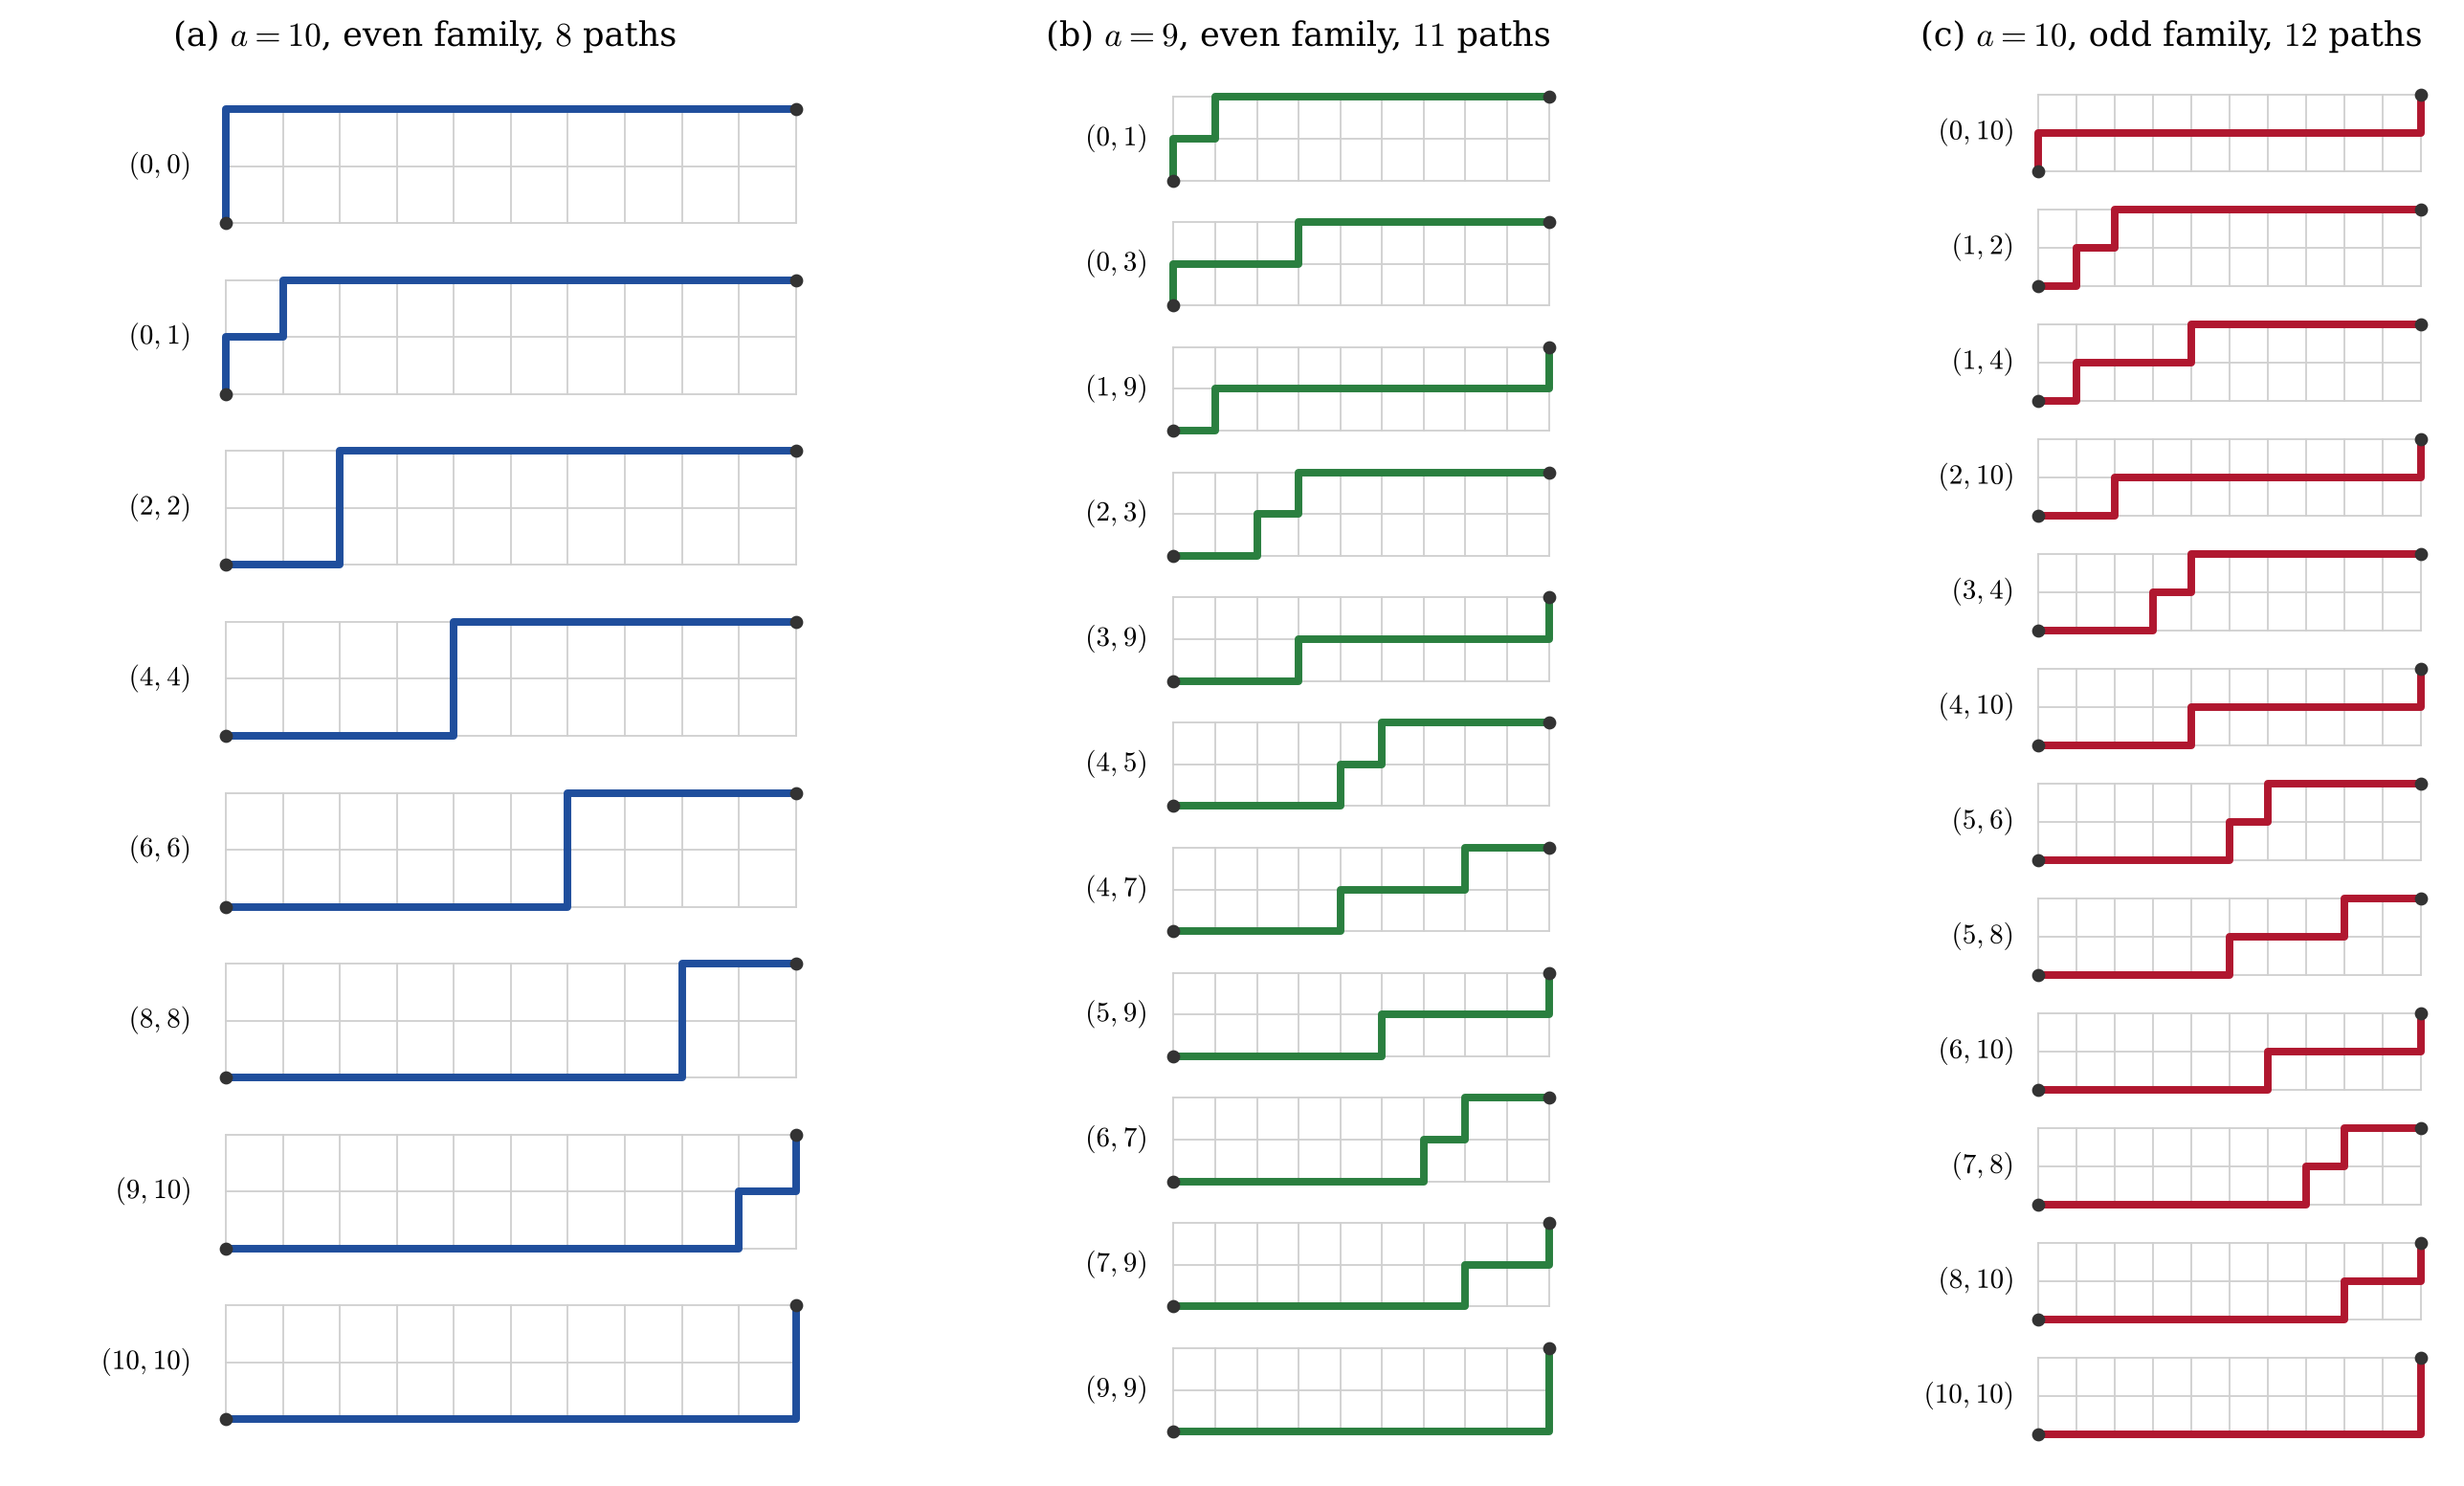
\includegraphics[width=\textwidth]{fig_tworows.png}
\caption{The families of Theorem~\ref{thm:tworows}, each path drawn in its own copy of the $a\times2$ grid and labelled by the positions $(i,i')$ of its north steps: (a) the one-class family for $a=10$, whose vertical double steps stand on the even lines and which is completed by $(0,1)$ and $(9,10)$; (b) the even family for $a=9$, made of the short steps $(2j,2j+1)$, the longer steps $(4t,4t+3)$ and the paths that end with a north step on the right side; (c) its shift for $a=10$, completed by $(0,10)$.}
\label{fig:tworows}
\end{figure}

\begin{proposition}\label{prop:tworowsexact}
For $2\le a\le22$ the bounds of Theorem~\ref{thm:tworows} are equalities.
\end{proposition}

The values come from the exhaustive search of Appendix~\ref{app:comp}, applied to the $\binom{a+2}{2}$ paths $(i,i')$ with the rules of Lemma~\ref{lem:tworows}. For comparison, Theorem~\ref{thm:D} gives only $4\le M_p(a,2)<2^{(a+2)/2}$ in the one-class case and $M_p(a,2)\le 2a+4-\gcd(a+1,3)$ in the other.\footnote{The rank of Theorem~\ref{thm:C} for $b=2$ is $r=2a-\gcd(a+1,3)+1$, and the bounds $r+3$ of Theorem~\ref{thm:D}(i) and $r+2$ of Theorem~\ref{thm:D}(ii) are at most $2a+4-\gcd(a+1,3)$. Theorem~\ref{thm:tworows} and Proposition~\ref{prop:tworowsexact} show that the true value is about $5a/4$, so for two rows the Gram matrix bound exceeds the truth by a factor close to $8/5$.} In the one-class construction all paths but two are vertical double steps on lines of one parity, which pairwise fall under case (A).

\subsection{Odd lengths and the Catalan numbers}

\begin{proof}[Proof of Theorem~\ref{thm:E}]
Let $M$ be a noncrossing perfect matching of $[2n+2]$, and let $\{p_0,2n+2\}$ be its arc through the last point. Let
\[
R_M=\{x\in L(2n+1):\ x1\in\cF_M\}.
\]
The words of $\cF_M$ ending in $1$ are exactly those with $x_{p_0}=0$, so $|R_M|=2^{n+1}/2=2^n$, and every word of $R_M$ has weight $n$; so $R_M$ is a family of paths from $(0,0)$ to $(n+1,n)$. For distinct $x,y\in R_M$, Lemma~\ref{lem:basic}(b) and Theorem~\ref{thm:A} give
\[
0=B_{2n+2}(x1,y1)=B_{2n+1}(x,y)+1,
\]
so $B_{2n+1}(x,y)=1$ and $R_M$ is an odd family.

The matching can be recovered from $R_M$. The words of $R_M$ are the words $x\in L(2n+1)$ with $x_{p_0}=0$ and $x_p\ne x_q$ for the arcs $\{p,q\}$ of $M$ inside $[2n+1]$. Position $p_0$ is the only position at which all words of $R_M$ agree, and as in the proof of Proposition~\ref{prop:skeleton} two positions of $[2n+1]\setminus\{p_0\}$ carry different letters in every word of $R_M$ exactly when they form an arc of $M$. So $M\mapsto R_M$ is injective, and there are at least $C_{n+1}$ distinct odd families of size $2^n$. The upper bound $\Modd(n+1,n)<2^{(2n+1)/2}$ is Theorem~\ref{thm:D}(ii).
\end{proof}

By reversing words, which rotates every path by a half turn and preserves common edges, and by exchanging letters, the same holds for paths from $(0,0)$ to $(n,n+1)$. Figure~\ref{fig:oddcat} shows the construction for $n=2$.

\begin{figure}[ht]
\centering
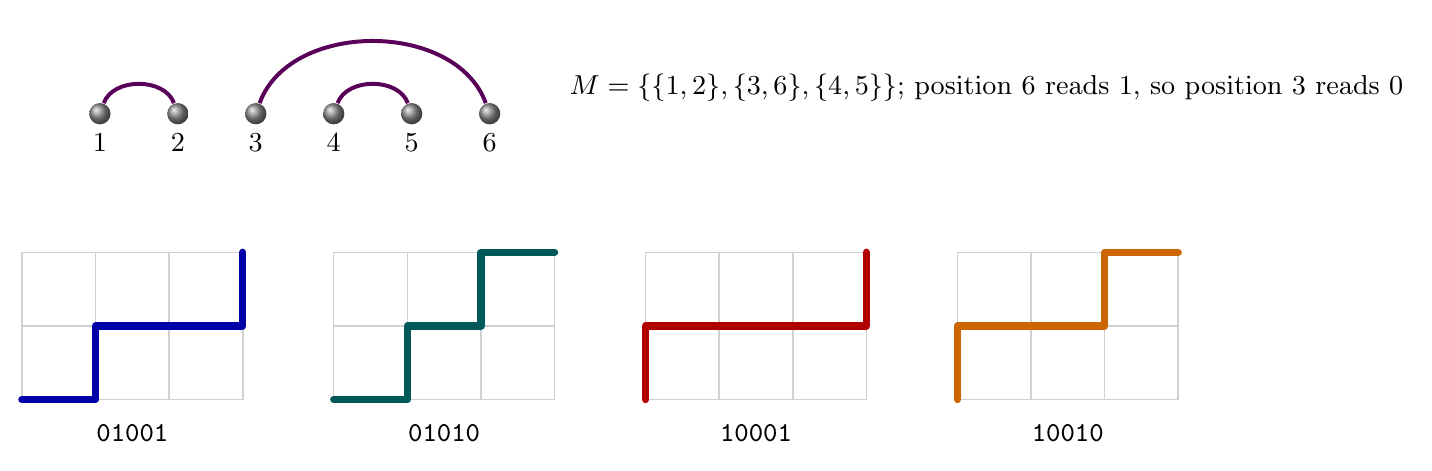
\includegraphics[width=0.9\textwidth]{fig_oddcat.png}
\caption{Theorem~\ref{thm:E} for $n=2$. The matching $M=\{\{1,2\},\{3,6\},\{4,5\}\}$ of $[6]$ gives the eight paths of $\cF_M$ from $(0,0)$ to $(3,3)$; the four that end with a north step, with that step removed, form an odd family of paths from $(0,0)$ to $(3,2)$. Any two of the four share one or three edges.}
\label{fig:oddcat}
\end{figure}

\subsection{Odd families in the square}

Shankar's lower bounds for $\Modd(n,n)$ are $k^2$ for $n=2k$ and $k(k+2)$ for $n=2k+1$~\cite{Sh}. The exact values for small $n$ are larger.

\begin{proposition}\label{prop:oddsmall}
The values of $\Modd(n,n)$ for $n=1,\dots,6$ are $1$, $2$, $3$, $6$, $10$ and $16$, while $\Modd(7,7)\ge20$ and $\Modd(8,8)\ge28$.
\end{proposition}

The exact values come from the exhaustive search described in Appendix~\ref{app:comp}, and the families for $n=6,7,8$ are listed in Appendix~\ref{app:families}, where their odd intersections can be checked by hand with~\eqref{eq:common}. For $n=6,7,8$ these numbers exceed the constructions of~\cite{Sh}, which give $9$, $15$ and $16$, by $7$, $5$ and $12$; for $n=3,4,5$ the exact value, and for $n=8$ the lower bound, equals $\binom n2$. Figure~\ref{fig:oddvalues} compares the known values with the two bounds.

\begin{figure}[ht]
\centering
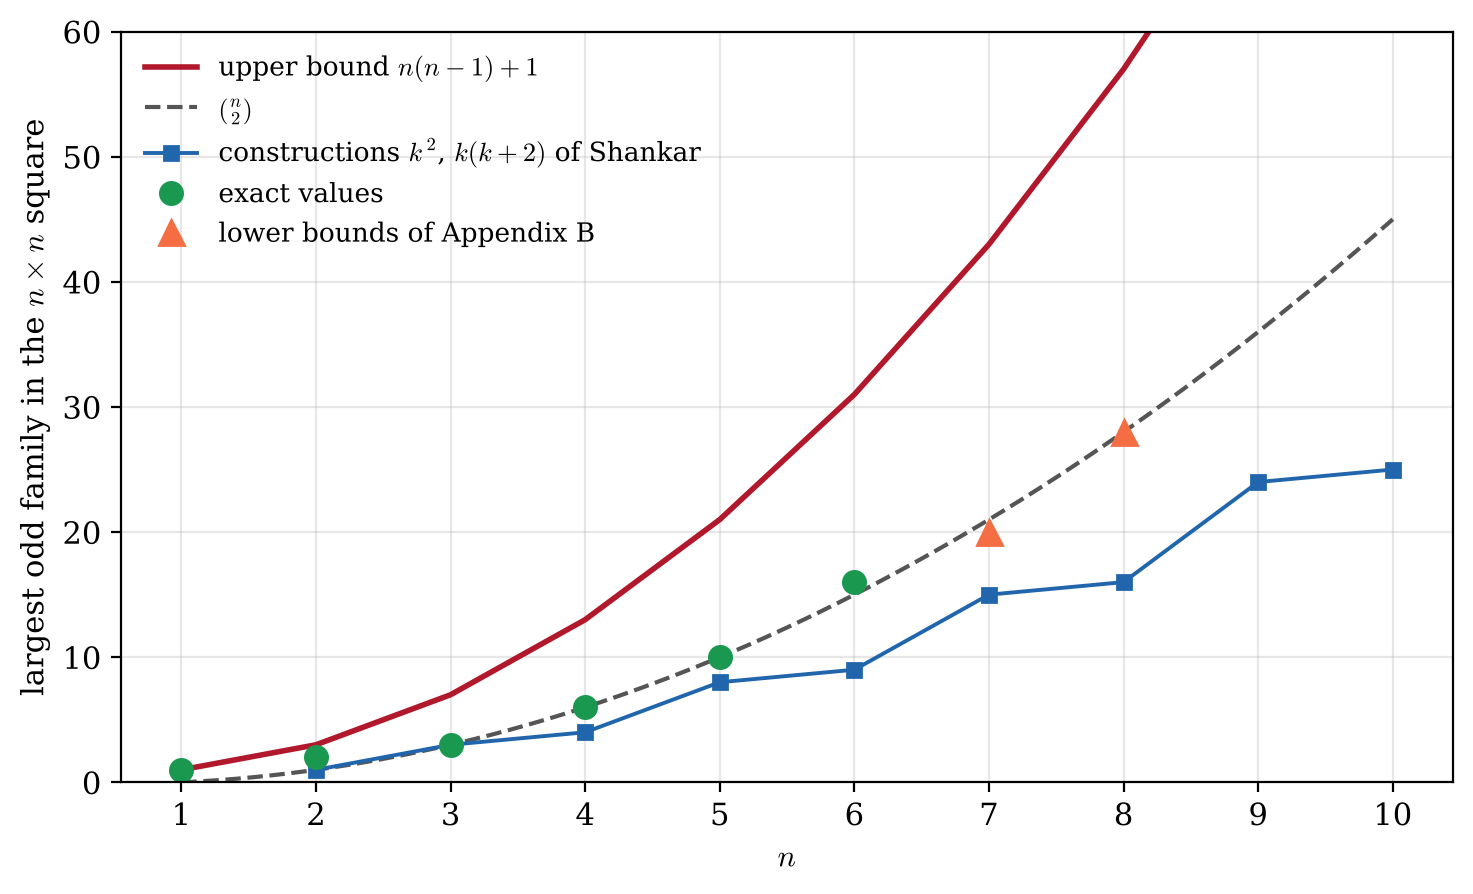
\includegraphics[width=0.8\textwidth]{fig_oddvalues.png}
\caption{Odd families in the square: the exact values of $\Modd(n,n)$ for $n\le6$ and the lower bounds for $n=7,8$ (dots), Shankar's upper bound $n(n-1)+1$, his constructions $k^2$ and $k(k+2)$, and the curve $\binom n2$.}
\label{fig:oddvalues}
\end{figure}

Call a path \emph{unit} if every maximal run of north steps that is neither the first nor the last run of its word has length $1$. The families for $n=7$ and $n=8$ in Appendix~\ref{app:families} were found by an exact search among unit paths: there are $320$ of them for $n=7$ and $704$ for $n=8$, against $3432$ and $12870$ paths in all.

\section{Open problems}\label{sec:open}

\begin{conjecture}\label{conj:oddcatalan}
For every $n\ge1$, $\Modd(n+1,n)=2^n$, and the odd families of size $2^n$ of paths from $(0,0)$ to $(n+1,n)$ are exactly the $C_{n+1}$ families $R_M$ of Theorem~\ref{thm:E}.
\end{conjecture}

The value is confirmed for $n\le5$ and the count for $n\le4$. The first part has an equivalent form in terms of admissible systems. Splitting an odd family $\cF$ by its last letter, $\cF=X0\cup Y1$, Lemma~\ref{lem:basic}(b) shows that $X$ and $Y$ are even families of words of length $2n$ and weights $n$ and $n-1$, and that $B_{2n}(x,y)=B_{2n+1}(x0,y1)=1$ for $x\in X$ and $y\in Y$; so $\{X,Y\}$ (without the empty sets) is an admissible system of length $2n$. Conversely, for every admissible system $\{X,Y\}$ of length $2n$ with weights $n$ and $n-1$ and $B_{2n}\equiv1$ on $X\times Y$, the set $X0\cup Y1$ is an odd family. Hence $\Modd(n+1,n)=2^n$ if and only if $|X|+|Y|\le2^n$ for all such systems. Proposition~\ref{prop:inequality} gives only $|X|^2+|Y|^2\le2^{2n}$, and Remark~\ref{rem:classsizes} shows that equality cannot hold when both sets are nonempty; the conjecture asks for the stronger, linear form of this inequality.

The first part of Conjecture~\ref{conj:oddcatalan} is the constant-weight case of a statement about paths of odd length whose endpoints are not fixed.

\begin{conjecture}\label{conj:freeend}
Let $m$ be odd, and let $\cF$ be a set of lattice paths of length $m$ starting at $(0,0)$, with arbitrary endpoints, in which every two distinct paths share an odd number of edges. Then $|\cF|\le2^{(m-1)/2}$.
\end{conjecture}

In terms of words, $\cF\subseteq L(m)$ and $B_m(x,y)=1$ for all distinct $x,y\in\cF$. The bound is attained, for instance by the families of Theorem~\ref{thm:E}, and also by families whose endpoints differ (Figure~\ref{fig:freeend}).

\begin{figure}[ht]
\centering
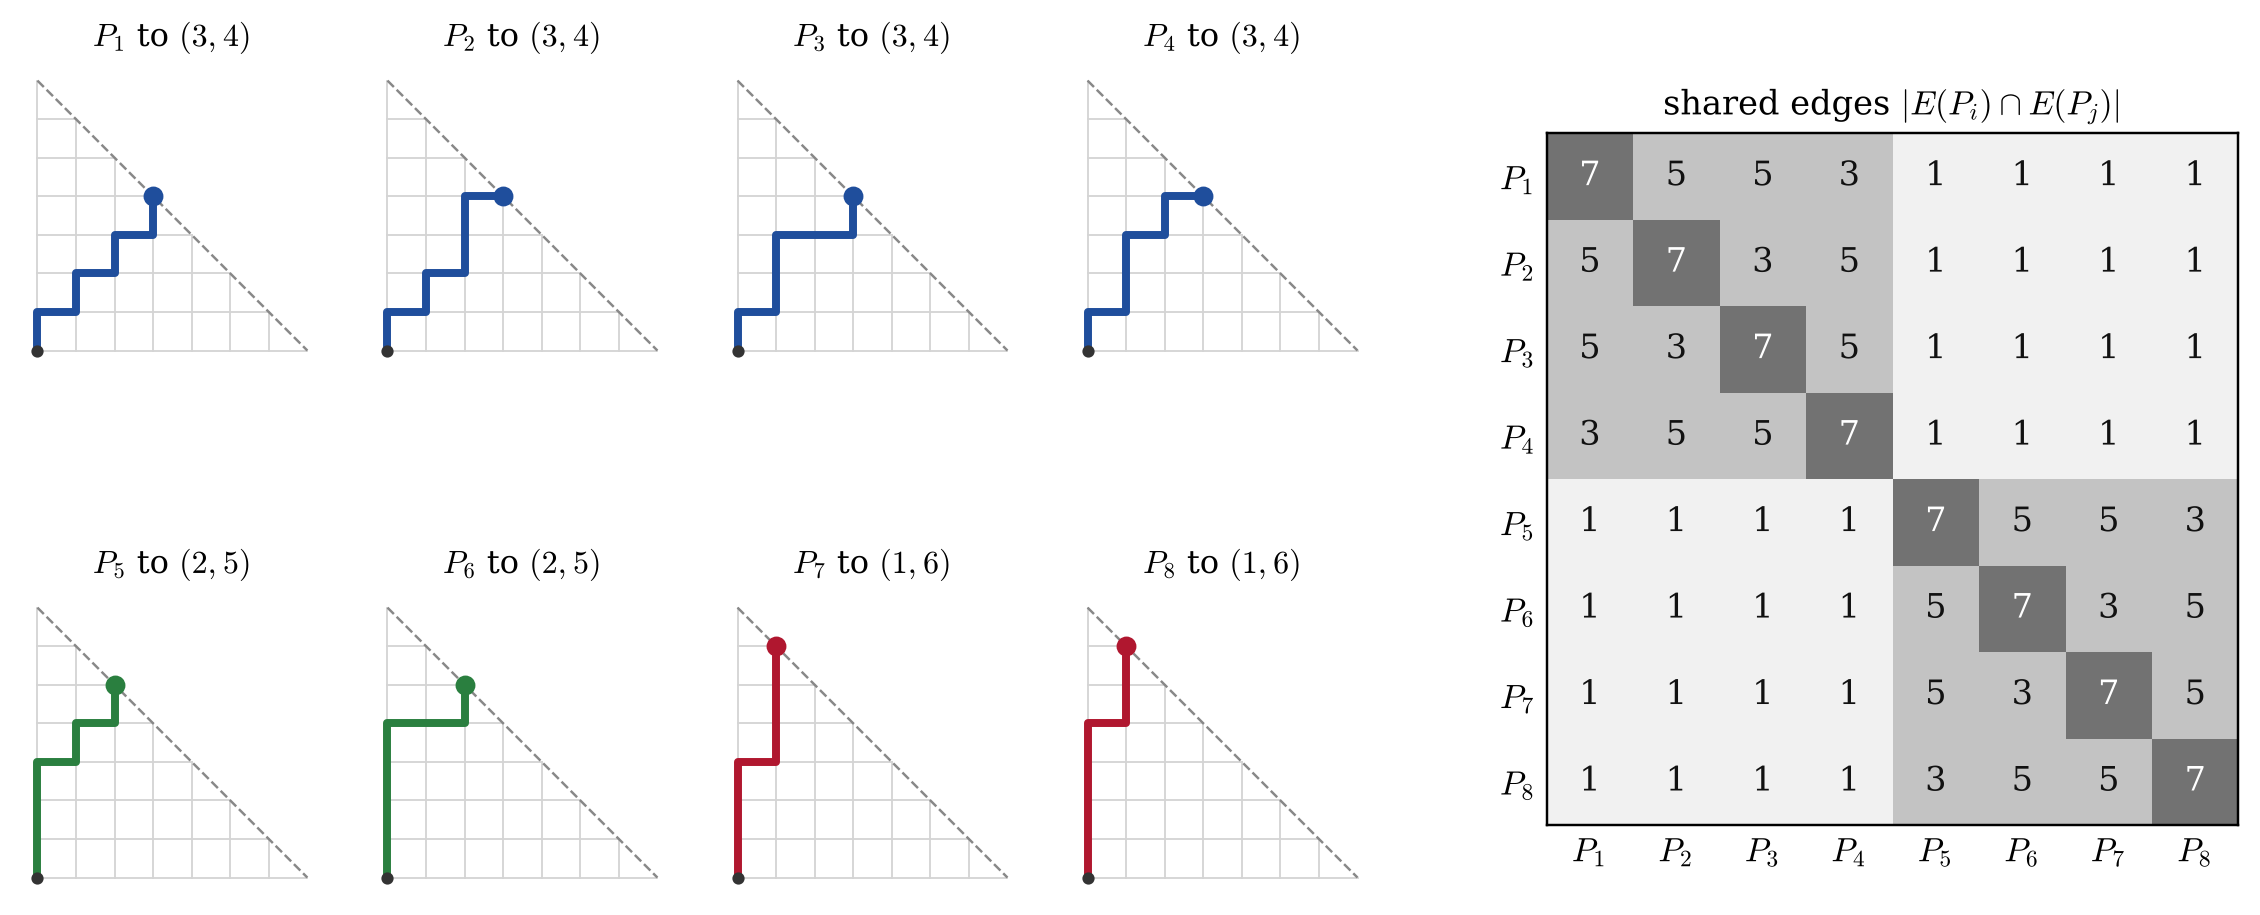
\includegraphics[width=\textwidth]{fig_freeend.png}
\caption{Eight paths of length $7$ from $(0,0)$ with three different endpoints, every two of which share an odd number of edges; the matrix on the right lists the numbers of shared edges. The family has the largest size $2^{3}$ allowed by Conjecture~\ref{conj:freeend}.}\label{fig:freeend}
\end{figure}

\begin{proposition}\label{prop:freeend}
For $k\ge0$ let $f(k)$ be the largest size of a set $\cF\subseteq L(2k+1)$ whose words all have weights of the same parity and satisfy $B_{2k+1}(x,y)=1$ for $x\ne y$, and let $h(k)$ be the largest size of a set $\cG\subseteq L(2k)$ with
\[
B_{2k}(u,v)=\Iv{\wt(u)\ne\wt(v)}\qquad\text{for all distinct }u,v\in\cG .
\]
Then $f(k)=h(k)$. If Conjecture~\ref{conj:freeend} holds for $m=2k-1$, then $h(k)\le2^k$. Consequently Conjecture~\ref{conj:freeend} for $m=2n-1$ implies $\Modd(n+1,n)=2^n$.
\end{proposition}

\begin{proof}
Let $\cF$ be as in the definition of $f(k)$, with all weights congruent to $p$ modulo $2$, and write $\cF=X0\cup Y1$. If $u0$ and $u1$ both lay in $\cF$, Lemma~\ref{lem:basic} would give $B_{2k+1}(u0,u1)=B_{2k}(u,u)=0$; hence $X\cap Y=\varnothing$. Words of $X$ have weights congruent to $p$ and words of $Y$ weights congruent to $p+1$. For distinct $u,v\in X$, Lemma~\ref{lem:basic} gives $1=B_{2k+1}(u0,v0)=B_{2k}(u,v)+\Iv{\wt(u)=\wt(v)}$, so $B_{2k}(u,v)=\Iv{\wt(u)\ne\wt(v)}$; the same holds in $Y$. For $u\in X$ and $v\in Y$, $B_{2k}(u,v)=B_{2k+1}(u0,v1)=1=\Iv{\wt(u)\ne\wt(v)}$, since the weights have different parities. So $\cG=X\cup Y$ is as in the definition of $h(k)$, and $|\cG|=|\cF|$. Conversely, for such a $\cG$ the set $\{u0:\ \wt(u)\equiv p\}\cup\{u1:\ \wt(u)\not\equiv p\}$ has $|\cG|$ elements, all of weight congruent to $p$, and the same computation read backwards gives $B_{2k+1}=1$ on distinct pairs. Hence $f(k)=h(k)$.

Let $k\ge1$ and let $\cG$ be as in the definition of $h(k)$. For $e\in\{0,1\}$ put $\cG_e=\{v\in L(2k-1):\ ve\in\cG\}$. For distinct $u,v\in\cG_e$,
\[
B_{2k-1}(u,v)=B_{2k}(ue,ve)+\Iv{\wt(u)=\wt(v)}=\Iv{\wt(u)\ne\wt(v)}+\Iv{\wt(u)=\wt(v)}=1,
\]
because $ue$ and $ve$ have different weights exactly when $u$ and $v$ do. So $\cG_e$ satisfies the hypothesis of Conjecture~\ref{conj:freeend} with $m=2k-1$, and $|\cG|=|\cG_0|+|\cG_1|\le2\cdot2^{k-1}$. An odd family of paths from $(0,0)$ to $(n+1,n)$ is a set as in the definition of $f(n)$, so $\Modd(n+1,n)\le f(n)=h(n)\le2^n$, and Theorem~\ref{thm:E} gives equality.
\end{proof}

The search of Appendix~\ref{app:comp}, run on the graph of all words of length $m$, confirms Conjecture~\ref{conj:freeend} for $m\le9$, and $f(k)=2^k$ for $k\le5$.\footnote{The natural induction removes the last two letters. Write $\cF_{st}=\{u:\ ust\in\cF\}$ for $s,t\in\{0,1\}$. By Lemma~\ref{lem:basic}, $B_m(ust,vs't')=B_{m-2}(u,v)$ whenever $s\ne s'$ and $t\ne t'$, and also when $(s,t)=(s',t')$; so $\cF_{00}\cup\cF_{11}$ and $\cF_{01}\cup\cF_{10}$ again satisfy the hypothesis of Conjecture~\ref{conj:freeend}, now for length $m-2$. This gives $|\cF|\le2^{(m-1)/2}+|\cF_{00}\cap\cF_{11}|+|\cF_{01}\cap\cF_{10}|$, and the conjecture would follow if the two intersections were empty. They need not be: $u00$ and $u11$ share the odd number $m-2$ of edges. A sum-of-squares argument in the style of Proposition~\ref{prop:inequality} cannot replace this step, because the extremal families of Theorem~\ref{thm:E} split by their last letter as $(2^n,0)$ and as $(2^{n-1},2^{n-1})$, and no single quadratic bound is sharp at both points.}

Semidefinite bounds separate the two settings. Call two paths of the same length compatible when they share an odd number of edges, and join incompatible paths by an edge. An odd family is then an independent set, so the Lov\'asz number $\vartheta$ of this graph~\cite{Lo} bounds its size. For the paths from $(0,0)$ to $(n+1,n)$ the computed value of $\vartheta$ is $2^n$ for $n\le4$, which indicates that for these $n$ the first part of Conjecture~\ref{conj:oddcatalan} can be proved by an orthonormal representation; we have not found one that works for every $n$.\footnote{The values of $\vartheta$ were obtained by semidefinite programming, as described in Appendix~\ref{app:comp}. For $n\le3$ there is even a partition of the paths into $2^n$ even families, which proves the bound at once, since an odd family meets each even family at most once. Such partitions cannot exist for large $n$ if, as the values of Table~\ref{tab:values} suggest, $\Meven(n+1,n)$ grows polynomially: the $\binom{2n+1}{n}$ paths would need classes of average size $\binom{2n+1}{n}2^{-n}$, which grows exponentially.} For paths with free endpoints the same bound is not sharp: for $m=5$ it is about $4.41$, while the largest family has $4$ members.

Theorem~\ref{thm:D}(iii) gives $\Modd(n+1,n)\ge\Meven(n,n)$, and the computations suggest that the passage from length $2n$ to length $2n+1$ never helps, in every rectangle. Call a family of paths from $(0,0)$ to $(a,b)$ \emph{one-class} if it is even when $a+b$ is even and odd when $a+b$ is odd, and let $g(a,b)$ be the largest size of such a family.

\begin{conjecture}\label{conj:shift}
If $a\ge b\ge1$ and $a-b$ is even, then $g(a+1,b)=g(a,b)$.
\end{conjecture}

For $a=b=n$ this is the first part of Conjecture~\ref{conj:oddcatalan}. Theorem~\ref{thm:D}(iii) gives $g(a+1,b)\ge g(a,b)$, and equality holds whenever both values appear in Table~\ref{tab:values} and, by Proposition~\ref{prop:tworowsexact}, for $b=2$ and $a\le21$. Proposition~\ref{prop:onerow} proves it for $b=1$, where $g(a,1)=2$ for all $a$.

\begin{conjecture}\label{conj:tworows}
The bounds of Theorem~\ref{thm:tworows} are equalities for every $a\ge2$.
\end{conjecture}

The one-class part of Conjecture~\ref{conj:tworows} reads $g(a,2)=\lfloor a/2\rfloor+3$, which would prove Conjecture~\ref{conj:shift} for $b=2$. Deleting the first and the last column of the grid maps the one-class paths $(i,i')$ with $1\le i\le i'\le a-1$ to one-class paths from $(0,0)$ to $(a-2,2)$, since every pair loses exactly two common edges. By Lemma~\ref{lem:tworows}(B) and (C), no three paths of a one-class family share their first north step, and no three share their second. Hence $g(a,2)\le g(a-2,2)+4$, which falls short of the conjectured increment $1$. A covering argument cannot close the gap: for $a=7,8,9$ the paths cannot be split into $\lfloor a/2\rfloor+3$ sets of pairwise incompatible paths. The semidefinite bound $\vartheta'$ of Schrijver~\cite{Sc}, however, equals $\lfloor a/2\rfloor+3$ for every $a\le10$, which points to a proof by a quadratic inequality.

\begin{problem}\label{prob:oddsquare}
Determine the order of $\Modd(n,n)/n^2$. Is $\Modd(n,n)\ge\binom n2$ for every $n\ge3$?
\end{problem}

The upper bound of Theorem~\ref{thm:D} is $n^2-n+1$ and the best general construction gives about $n^2/4$; the values of Proposition~\ref{prop:oddsmall} suggest $\tfrac12$ as the true constant.

\begin{problem}\label{prob:even}
Determine $\Meven(a,b)$ for $a\ne b$ with $a+b$ even.
\end{problem}

Theorem~\ref{thm:D} gives $2^{\min(a,b)}\le\Meven(a,b)<2^{(a+b)/2}$, and neither bound is the truth in general: the computed values are $\Meven(n+2,n)=2,5,10,21,42$ for $n=1,\dots,5$, which equal $\lfloor 2^{n+2}/3\rfloor$. We conjecture that $\Meven(n+2,n)=\lfloor 2^{n+2}/3\rfloor$ for all $n\ge1$. The same numbers appear as $\Modd(n+3,n)$ for $n\le4$, as Conjecture~\ref{conj:shift} predicts. For $b=1$ the problem is solved by Proposition~\ref{prop:onerow}, and for $b=2$ Theorem~\ref{thm:tworows} and Proposition~\ref{prop:tworowsexact} give the values for $a\le22$ and the lower bounds for all $a$.

\begin{problem}\label{prob:delta}
Characterise the pairs $(a,b)$ with $a+b$ even for which $q$ lies in the column space of $A_{a,b}$, that is $\delta(a,b)=0$.
\end{problem}

The computations of Table~\ref{tab:delta} show $\delta(a,b)=0$ when $a$ and $b$ are both even and when $a=b$, and for odd $a\ne b$ they show $\delta(a,b)=0$ exactly when $a\equiv b\equiv1\pmod4$ in the range $a,b\le10$.

\appendix

\section{Computations}\label{app:comp}

No proof in this paper depends on a computation; the computations below supply the exact values quoted in Propositions~\ref{prop:oddsmall} and~\ref{prop:tworowsexact}, in~\eqref{eq:transferobs}, in Section~\ref{sec:open} and in Table~\ref{tab:delta}, and they check the theorems on small cases.

\subsection*{Maximum families}
For given $a$, $b$ and parity $p$, let $\mathcal{H}$ be the graph on the $\binom{a+b}{b}$ paths from $(0,0)$ to $(a,b)$ in which two paths are adjacent when the parity of their number of common edges is $p$, computed by~\eqref{eq:common}. A family with the required parity is a clique of $\mathcal H$, so $\Meven(a,b)$ and $\Modd(a,b)$ are clique numbers. They were computed by an exact branch-and-bound search on bit sets, which orders the vertices greedily, bounds each branch by the number of colours of a greedy colouring of the candidate set, and discards a branch when this bound cannot beat the best clique found so far. The search is exhaustive and returns a clique of maximum size, which was then checked pair by pair. Table~\ref{tab:values} lists the results for $1\le b\le a\le 7$ and $a+b\le12$; the values for $a=b\le6$ give the first part of Proposition~\ref{prop:oddsmall}.

\begin{table}[ht]
\centering
\caption{Exact values of $\Meven(a,b)$ and $\Modd(a,b)$; $\binom{a+b}{b}$ is the number of paths.}
\label{tab:values}
\small
\begin{tabular}{ccccc@{\qquad}ccccc}
\toprule
$(a,b)$ & $a+b$ & $\binom{a+b}{b}$ & $\Meven$ & $\Modd$ & $(a,b)$ & $a+b$ & $\binom{a+b}{b}$ & $\Meven$ & $\Modd$\\
\midrule
$(1,1)$ & 2 & 2 & 2 & 1 & $(5,3)$ & 8 & 56 & 10 & 7 \\
$(2,1)$ & 3 & 3 & 2 & 2 & $(5,4)$ & 9 & 126 & 10 & 16 \\
$(2,2)$ & 4 & 6 & 4 & 2 & $(5,5)$ & 10 & 252 & 32 & 10 \\
$(3,1)$ & 4 & 4 & 2 & 2 & $(6,1)$ & 7 & 7 & 4 & 2 \\
$(3,2)$ & 5 & 10 & 3 & 4 & $(6,2)$ & 8 & 28 & 6 & 7 \\
$(3,3)$ & 6 & 20 & 8 & 3 & $(6,3)$ & 9 & 84 & 10 & 10 \\
$(4,1)$ & 5 & 5 & 3 & 2 & $(6,4)$ & 10 & 210 & 21 & 11 \\
$(4,2)$ & 6 & 15 & 5 & 4 & $(6,5)$ & 11 & 462 & 16 & 32 \\
$(4,3)$ & 7 & 35 & 6 & 8 & $(6,6)$ & 12 & 924 & 64 & 16 \\
$(4,4)$ & 8 & 70 & 16 & 6 & $(7,1)$ & 8 & 8 & 2 & 4 \\
$(5,1)$ & 6 & 6 & 2 & 3 & $(7,2)$ & 9 & 36 & 8 & 6 \\
$(5,2)$ & 7 & 21 & 6 & 5 & $(7,3)$ & 10 & 120 & 12 & 11 \\
 & & & & & $(7,4)$ & 11 & 330 & 15 & 21 \\
 & & & & & $(7,5)$ & 12 & 792 & 42 & 18 \\
\bottomrule
\end{tabular}
\end{table}

The table agrees with every statement of the paper that it touches: $\Meven(n,n)=2^n$ (Theorem~\ref{thm:A}); $\Modd(n+1,n)=2^n$ for $n\le5$ (Conjecture~\ref{conj:oddcatalan}); the values for $b=1$ (Proposition~\ref{prop:onerow}); and the bounds of Theorem~\ref{thm:D}. For example $\Meven(4,2)=5$ lies strictly between $2^2$ and $2^3$, and $\Modd(7,4)=21$ lies between $2^4$ and $2^{11/2}$.

\subsection*{Counting extremal families}
Listing all maximal cliques of $\mathcal H$ shows that the even families of $2^n$ paths in the $n\times n$ square number $1,2,5,14$ for $n=1,2,3,4$, as Theorem~\ref{thm:A} predicts, and that the odd families of $2^n$ paths from $(0,0)$ to $(n+1,n)$ number $2,5,14,42$ for $n=1,2,3,4$, which are $C_2,\dots,C_5$; by Theorem~\ref{thm:E} they are exactly the families $R_M$.

\subsection*{Odd families in larger squares}
For $n=7,8$ the full search is too slow, and the search was restricted to unit paths (Section~\ref{sec:rect}). Among the $320$ unit paths from $(0,0)$ to $(7,7)$ the largest odd family has $20$ members, and among the $704$ unit paths from $(0,0)$ to $(8,8)$ it has $28$. These give the lower bounds of Proposition~\ref{prop:oddsmall}.

\subsection*{Paths with free endpoints}
For Conjecture~\ref{conj:freeend} the same search was run on the graph of all $2^m$ words of length $m$, two words being adjacent when $B_m=1$. Its clique number is $1,2,4,8,16$ for $m=1,3,5,7,9$, which is $2^{(m-1)/2}$. Restricted to the words of length $2k+1$ whose weights have a fixed parity, the search gives $f(k)=1,2,4,8,16,32$ for $k=0,\dots,5$, for both parities. Figure~\ref{fig:freeend} shows one of the largest families for $m=7$.

\subsection*{Semidefinite bounds}
The Lov\'asz number $\vartheta$ and Schrijver's number $\vartheta'$ of Section~\ref{sec:open} were computed as the optimum of the standard semidefinite programs~\cite{Lo,Sc} with an interior point solver. For the paths from $(0,0)$ to $(n+1,n)$, $\vartheta=4,8,16$ for $n=2,3,4$; for all words of length $5$, $\vartheta\approx4.412$; and for the one-class problem in the $a\times2$ rectangle, $\vartheta'=\lfloor a/2\rfloor+3$ for $4\le a\le10$. The partitions into $2^n$ even families for $n\le3$, and the nonexistence of partitions into $\lfloor a/2\rfloor+3$ sets of pairwise incompatible paths for $a=7,8,9$, were found by a satisfiability solver.

\subsection*{Two rows}
For $b=2$ the graph $\mathcal H$ was built on the $\binom{a+2}2$ pairs $(i,i')$, with adjacency read off from Lemma~\ref{lem:tworows} and checked against a direct count of common edges, and its clique number was computed by the same search for $2\le a\le22$ and both parities. The results are, for $a=2,3,\dots,22$,
\begin{align*}
\Meven(a,2)&=4,3,5,6,6,8,7,11,8,13,9,16,10,18,11,21,12,23,13,26,14,\\
\Modd(a,2)&=2,4,4,5,7,6,9,7,12,8,14,9,17,10,19,11,22,12,24,13,27,
\end{align*}
which are the bounds of Theorem~\ref{thm:tworows}. The families of the theorem were also checked by a direct count of common edges for $a\le60$.

\subsection*{The rank of the Gram matrix}
Gaussian elimination over $\F_2$ confirms Theorem~\ref{thm:C} for all $a,b\le12$ and gives the values of $\delta(a,b)$ in Table~\ref{tab:delta}.

\begin{table}[ht]
\centering
\caption{The value of $\delta(a,b)$ for $a,b\le10$ with $a+b$ even ($\cdot$ when $a+b$ is odd). Here $\delta(a,b)=0$ exactly when $q$ lies in the column space of $A_{a,b}$.}
\label{tab:delta}
\small
\begin{tabular}{c|cccccccccc}
$a\backslash b$ & 1 & 2 & 3 & 4 & 5 & 6 & 7 & 8 & 9 & 10\\
\hline
1 & 0 & $\cdot$ & 1 & $\cdot$ & 0 & $\cdot$ & 1 & $\cdot$ & 0 & $\cdot$ \\
2 & $\cdot$ & 0 & $\cdot$ & 0 & $\cdot$ & 0 & $\cdot$ & 0 & $\cdot$ & 0 \\
3 & 1 & $\cdot$ & 0 & $\cdot$ & 1 & $\cdot$ & 1 & $\cdot$ & 1 & $\cdot$ \\
4 & $\cdot$ & 0 & $\cdot$ & 0 & $\cdot$ & 0 & $\cdot$ & 0 & $\cdot$ & 0 \\
5 & 0 & $\cdot$ & 1 & $\cdot$ & 0 & $\cdot$ & 1 & $\cdot$ & 0 & $\cdot$ \\
6 & $\cdot$ & 0 & $\cdot$ & 0 & $\cdot$ & 0 & $\cdot$ & 0 & $\cdot$ & 0 \\
7 & 1 & $\cdot$ & 1 & $\cdot$ & 1 & $\cdot$ & 0 & $\cdot$ & 1 & $\cdot$ \\
8 & $\cdot$ & 0 & $\cdot$ & 0 & $\cdot$ & 0 & $\cdot$ & 0 & $\cdot$ & 0 \\
9 & 0 & $\cdot$ & 1 & $\cdot$ & 0 & $\cdot$ & 1 & $\cdot$ & 0 & $\cdot$ \\
10 & $\cdot$ & 0 & $\cdot$ & 0 & $\cdot$ & 0 & $\cdot$ & 0 & $\cdot$ & 0 \\
\end{tabular}
\end{table}

\section{Odd families in the square}\label{app:families}

The following families of paths from $(0,0)$ to $(n,n)$ are odd; a path is written as a word with $1$ for a north step and $0$ for an east step.

\medskip\noindent\emph{$n=6$, sixteen paths.}
\begin{center}\small\ttfamily
\begin{tabular}{llll}
111101100000 & 111111000000 & 111101001000 & 111010010100 \\
111000110100 & 110100010110 & 111000011100 & 110001010110 \\
101000010111 & 100010010111 & 100000111011 & 100000101111 \\
010000111110 & 001010011110 & 000100111110 & 000001111110 \\
\end{tabular}
\end{center}

\medskip\noindent\emph{$n=7$, twenty paths.}
\begin{center}\small\ttfamily
\begin{tabular}{llll}
11111110000000 & 11111100100000 & 11111100001000 & 11111001010000 \\
11111001000100 & 11111000010100 & 11111100000010 & 11110000101010 \\
11100101010100 & 11110010001010 & 11100100001011 & 11100001010011 \\
10101001000111 & 10100000011111 & 10010101010011 & 10010001001111 \\
10001000011111 & 10000101001111 & 10000010011111 & 10000000111111 \\
\end{tabular}
\end{center}

\medskip\noindent\emph{$n=8$, twenty-eight paths.}
\begin{center}\small\ttfamily
\begin{tabular}{llll}
1111111001000000 & 1111111100000000 & 1111111000010000 & 1111110010100000 \\
1111110000101000 & 1111110010001000 & 1111111000000100 & 1111100100010100 \\
1111100100000011 & 1111100000010011 & 1111001010101000 & 1110010100010011 \\
1110010001010011 & 1110010000001111 & 1110000001001111 & 1010101010101001 \\
1010101010000111 & 1010101000100111 & 1010100000011111 & 1010100010100111 \\
1010000010011111 & 1001010001001111 & 1000100010011111 & 1001000000111111 \\
1001000101001111 & 1000001010011111 & 1000000100111111 & 1000000001111111 \\
\end{tabular}
\end{center}

\begin{example}\label{ex:check}
In the family for $n=6$, the paths $111111000000$ and $000001111110$ meet only in the top edge from $(5,6)$ to $(6,6)$: the first runs up the left side and along the top, the second along the bottom to $(5,0)$, up the line $x=5$ and then one step east. By~\eqref{eq:common}, only position $12$ counts, since both words end with $0$ and both prefixes of length $11$ have weight $6$. The paths $111111000000$ and $111101100000$ share the four edges of the left side from $(0,0)$ to $(0,4)$ and the five top edges from $(1,6)$ to $(6,6)$, nine in all. Every other pair is checked in the same way.
\end{example}

\section*{Declarations}

\subsection*{Funding} This research received no funding.

\subsection*{Competing interests} The author declares that there are no competing interests.

\subsection*{Data availability} No external data sets were used. The exact values in Appendix~\ref{app:comp} were obtained by the exhaustive search described there and can be reproduced from that description; the programs that perform the search, check the families of Theorem~\ref{thm:tworows} and test Conjecture~\ref{conj:freeend} are included with this preprint as supplementary files. The families in Appendix~\ref{app:families} are printed in full.

\subsection*{Use of artificial intelligence} AI coding assistants were used to write and test the search programs and to check the bibliography. All mathematical arguments were written and verified by the author, who takes full responsibility for the content.

\subsection*{Acknowledgements} The problems treated here were posed by Umesh Shankar~\cite{Sh}, whose bounds, constructions, basis of the path space and conjecture are the starting point of this work; the notion of intersection of lattice paths through common edges is due to Hiranya Dey.

\raggedbottom
\begin{thebibliography}{99}

\bibitem{Be}
E.~R. Berlekamp, \emph{On subsets with intersections of even cardinality}, Canad. Math. Bull. \textbf{12} (1969), 471--474. \doi{10.4153/CMB-1969-059-3}

\bibitem{De}
E.~Deutsch, \emph{Dyck path enumeration}, Discrete Math. \textbf{204} (1999), 167--202. \doi{10.1016/S0012-365X(98)00371-9}

\bibitem{FO}
P.~Frankl and A.~M. Odlyzko, \emph{On subsets with cardinalities of intersections divisible by a fixed integer}, European J. Combin. \textbf{4} (1983), 215--220. \doi{10.1016/S0195-6698(83)80014-6}

\bibitem{FW}
P.~Frankl and R.~M. Wilson, \emph{Intersection theorems with geometric consequences}, Combinatorica \textbf{1} (1981), 357--368. \doi{10.1007/BF02579457}

\bibitem{GKT}
J.~Goldwasser, W.~Klostermeyer and G.~Trapp, \emph{Characterizing switch-setting problems}, Linear Multilinear Algebra \textbf{43} (1997), 121--135. \doi{10.1080/03081089708818520}

\bibitem{Gr}
J.~E. Graver, \emph{Boolean designs and self-dual matroids}, Linear Algebra Appl. \textbf{10} (1975), 111--128. \doi{10.1016/0024-3795(75)90003-8}

\bibitem{HJ}
R.~A. Horn and C.~R. Johnson, \emph{Matrix Analysis}, 2nd ed., Cambridge University Press, Cambridge, 2013. \doi{10.1017/CBO9781139020411}

\bibitem{HL}
V.~E. Hoggatt and C.~T. Long, \emph{Divisibility properties of generalized Fibonacci polynomials}, Fibonacci Quart. \textbf{12} (1974), 113--120. \doi{10.1080/00150517.1974.12430744}

\bibitem{Kr}
C.~Krattenthaler, \emph{Lattice path enumeration}, in: M.~B\'ona (ed.), \emph{Handbook of Enumerative Combinatorics}, Chapman and Hall/CRC, Boca Raton, 2015. \doi{10.1201/b18255-16}

\bibitem{Kre}
G.~Kreweras, \emph{Sur les partitions non crois\'ees d'un cycle}, Discrete Math. \textbf{1} (1972), 333--350. \doi{10.1016/0012-365X(72)90041-6}

\bibitem{Lo}
L.~Lov\'asz, \emph{On the Shannon capacity of a graph}, IEEE Trans. Inform. Theory \textbf{25} (1979), 1--7. \doi{10.1109/TIT.1979.1055985}

\bibitem{Sc}
A.~Schrijver, \emph{A comparison of the Delsarte and Lov\'asz bounds}, IEEE Trans. Inform. Theory \textbf{25} (1979), 425--429. \doi{10.1109/TIT.1979.1056072}

\bibitem{Sh}
U.~Shankar, \emph{Oddtown and eventown theorems for lattice paths}, preprint, 2026. \href{https://arxiv.org/abs/2607.23117}{arXiv:2607.23117}

\bibitem{Si}
R.~Simion, \emph{Noncrossing partitions}, Discrete Math. \textbf{217} (2000), 367--409. \doi{10.1016/S0012-365X(99)00273-3}

\bibitem{St}
R.~P. Stanley, \emph{Catalan Numbers}, Cambridge University Press, Cambridge, 2015. \doi{10.1017/CBO9781139871495}

\bibitem{StEC2}
R.~P. Stanley, \emph{Enumerative Combinatorics, Volume 2}, Cambridge Stud. Adv. Math. \textbf{62}, Cambridge University Press, Cambridge, 1999. \doi{10.1017/CBO9780511609589}

\bibitem{Sutner89}
K.~Sutner, \emph{Linear cellular automata and the Garden-of-Eden}, Math. Intelligencer \textbf{11} (1989), no.~2, 49--53. \doi{10.1007/BF03023823}

\bibitem{Sutner00}
K.~Sutner, \emph{$\sigma$-automata and Chebyshev-polynomials}, Theoret. Comput. Sci. \textbf{230} (2000), 49--73. \doi{10.1016/S0304-3975(97)00242-9}

\end{thebibliography}

\end{document}
